\documentclass{scrbook}
\KOMAoptions{paper=a4, fontsize=12pt, chapterprefix=true, twoside=semi, DIV=classic, parskip=half}

\usepackage[T1]{fontenc}
\usepackage[sf]{noto}
\linespread{1.25}

\usepackage{scrlayer-scrpage}
\usepackage[fulladjust]{marginnote}
\usepackage{enumitem}

\KOMAoptions{headsepline=on, captions=besidetop, DIV=last}

\pagestyle{scrheadings}
%\automark[chapter]{chapter}
%\automark*[section]{}
\setkomafont{pagehead}{\color{RoyalBlue}\slshape\bfseries}
\renewcommand*{\chaptermarkformat}{\chapapp~\thechapter\autodot~--~}
\ofoot*{}
\cfoot*{\pagemark}

\addtokomafont{chapterprefix}{\itshape\color{white}}
\renewcommand*{\chapterformat}{\raggedleft\colorbox{RoyalBlue}{\parbox[b][66pt]{66pt}{\vfill\centering{\large\chapapp}\\[-6pt]\thechapter\vfill}}}
\renewcommand*{\chapterheadendvskip}{\pgfornament[width=\textwidth]{88}\par}

\renewcommand*{\sectionformat}{\colorbox{black}{\textcolor{white}{\thesection}}\enskip}
\makeatletter
\renewcommand*\sectionlinesformat[4]{\makebox[0pt][l]{\rule[-\fboxsep]{\textwidth}{1pt}}\@hangfrom{#3}\parbox[b]{0.85\textwidth}{\linespread{1}\selectfont#4}}
\makeatother

\usepackage{graphicx}
\usepackage[svgnames, dvipsnames]{xcolor}
\usepackage[many]{tcolorbox}
\usepackage{pgfornament}
\usepackage{amsmath,amssymb,amsthm}
\usepackage{bm}
\usepackage{physics}
\usepackage{siunitx}
\usepackage{mathtools}
\usepackage{mdframed}
\usepackage{lipsum}
\usepackage{microtype}
\usepackage{tabularx}
\usepackage{adjustbox}
\usepackage{subcaption}
\usepackage{parcolumns}
\usepackage{multicol}

\definecolor{mint}{rgb}{0.24, 0.71, 0.54}

\usepackage[lastexercise,answerdelayed]{exercise}
\renewcounter{Exercise}[chapter]
\renewcommand*{\theExercise}{\thechapter.\arabic{Exercise}}
\renewcommand*{\ExerciseHeader}{\textbf{\theExercise )}}
\renewcommand*{\AnswerHeader}{\noindent \textbf{\theExercise}}
\renewcommand*{\ExerciseSkipBefore}{\dimexpr.5\baselineskip}
\renewcommand*{\ExerciseSkipAfter}{\dimexpr.5\baselineskip}

\newmdenv[leftmargin = 0pt,
  innerleftmargin = 1em,
  innertopmargin = 0.5em,
  innerbottommargin = 1em,
  innerrightmargin = 1em,
  frametitlebelowskip = 0.75em,
  rightmargin = 0pt,
  linewidth= 1ex,
  skipabove = \baselineskip,
  skipbelow = \baselineskip,
  splittopskip = \baselineskip,
  topline = false,
  rightline = false,
  bottomline = false,
  nobreak = true,
  backgroundcolor=Mahogany!20,
  linecolor=Mahogany,
  frametitle={\sffamily Exercise(s)},
  frametitleaboveskip = 1em,
  frametitlebackgroundcolor=Mahogany!10]{exercisebox}

\usepackage{listings}
\lstdefinestyle{lstTeXstyle}{
    language=[latex]TeX, 
    basicstyle=\footnotesize\ttfamily,
    backgroundcolor=\color{Goldenrod!20},
    keywordstyle=\color{blue!80}\bfseries,
    commentstyle=\color{Green},
    breaklines=true,
    showstringspaces=false,
    numbers=none,
    belowskip=0pt,
    escapeinside={/*!}{!*/},
}
\lstset{style=lstTeXstyle}

\usepackage{hyperref}

\title{How to Reproduce this Book Exactly with \LaTeX}
\subtitle{A Self-contained Tutorial on Writing Mathematical Notes}
\author{C.~L.~Loi}
\lowertitleback{"How to Reproduce this Book Exactly with \LaTeX"\\
Copyright ©, C.~L.~Loi, 2025. All rights reserved.}

%\setcounter{tocdepth}{}
\allowdisplaybreaks

\begin{document}

\frontmatter
\maketitle
\tableofcontents
\mainmatter
\chapter{The Basic Set-up and Structure of a \LaTeX{} Book}

\paragraph{Introduction}
The first chapter discusses how to properly configure \LaTeX{} files and organize the content's structure so that we can generate our first readable \LaTeX{} book PDF. 

\section{Class, Commands, Options, and Packages}
\label{sec:komaopt}

\paragraph{Class}
For each \LaTeX{} document, we need to specify its \textit{class}. Throughout this book, we will use the \verb|scrbook| class provided by the \textbf{KOMA-Script}. To do so, we write \texttt{\textbackslash documentclass\{scrbook\}} at the very beginning (\textit{preamble}) of the main \TeX{} file. Although not explored in this book, some other notable classes that may be of use include \verb|beamer|, \verb|moderncv|, and \verb|article| (or \verb|scrartcl|).

\paragraph{Commands and Options} The \verb|scrbook| class provides several \textit{options} to customize the format of the book. We can either supply the arguments when declaring the class, or use the command \texttt{\textbackslash KOMAoptions} in the preamble. A \textit{command} works like a function in common programming languages and performs some specific action. Commands in \LaTeX{} are denoted by the backslash \verb|\| as the first character. In this book, we have used
\begin{lstlisting}
\KOMAoptions{paper=a4, fontsize=12pt, chapterprefix=true, twoside=semi, DIV=classic, parskip=half}
\end{lstlisting}
The arguments are typed inside the curly brackets \verb|{}| following the name of the command. Clearly, the \verb|paper| option requires the pages to be in A4 size while \verb|fontsize| indicates that the font is 12 pt large. The remaining options will be explained as we go through the later chapters.

\paragraph{Packages} To enable extra functionalities, we need to import \textit{packages}. We can write along the lines of \texttt{\textbackslash usepackage[<options>]\{<package\_name>\}} in the preamble to do so. We will not list all the required packages now at once, but only when they are needed. The first package we usually need is the \verb|fontenc| package with the \verb|T1| option, flagged inside a pair of square brackets.

\begin{exercisebox}
\begin{Exercise}
Try to import the \verb|fontenc| package with the \verb|T1| option as suggested above. There may not be any noticeable difference, but at least you should not be receiving errors.
\end{Exercise}
\begin{Exercise}
Also, try to use \texttt{\textbackslash documentclass[<options>]\{scrbook\}} instead of the \texttt{\textbackslash KOMAoptions} command to achieve the same class setting.
\end{Exercise}
\end{exercisebox}

\section{Structure Hierarchy}

\subsection{Chapters and (Sub-)Sections}

\paragraph{Chapters, Sections} As in any other book, the entire content is divided into \textit{chapters}, which in turn usually consist of several \textit{sections}. To mark the beginning of a chapter or section, we place the commands \texttt{\textbackslash chapter\{<chapter\_name>\}} or \texttt{\textbackslash section\{<section\_name>\}} within the \verb|document| environment, which contains the main content and is marked by a pair of \verb|begin| and \verb|end| declarations. The preamble has to be inserted before \verb|document|. So, to typeset the very first section at the start, we write
\begin{lstlisting}
<preamble before the main document>
\begin{document}
...
\chapter{The Basic Set-up and Structure of a \LaTeX{} Book}
...
\section{Class, Options, and Packages}
\paragraph{Class}
For each \LaTeX{} document, we need to specify its \textit{class}. Throughout this book, ...
...
\end{document}
\end{lstlisting}
The \LaTeX{} system updates the chapter/section's numbering internally. The \texttt{\textbackslash textit\{<text>\}} command presents the text in italic shape.

\paragraph{Subsections, Paragraphs} An attentive reader may have already figured out that it is possible to stack an extra layer (a \textit{subsection}) in the hierarchy. This is aptly done not long ago by the \texttt{\textbackslash subsection\{<section\_name>\}} command:
\begin{lstlisting}
\section{Structure Hierarchy}

\subsection{Chapters and (Sub-)Sections}

\paragraph{Chapters, Sections} As in any other book, the entire content is divided into \textit{chapters}, ...
\end{lstlisting}
He/she may also notice that we have used the \texttt{\textbackslash paragraph} command a few times to attach an unnumbered heading for each \textit{paragraph}. There are also starred versions like \texttt{\textbackslash chapter*\{<chapter\_name>\}}, \texttt{\textbackslash section*\{<section\_name>\}}, \texttt{\textbackslash subsection*\{<section\_name>\}}, and so on, which neither display nor increase the numbering/counters.

\subsection{Generating Table of Contents}

\paragraph{Table of Contents}
After establishing the structure of the book, it is convenient to generate a \textit{table of contents (TOC)} as well. In the \verb|scrbook| class, it is easily done by adding the command \texttt{\textbackslash tableofcontents} within the main \verb|document| group. To control the depth of layers shown, we can call \texttt{\textbackslash setcounter{tocdepth}\allowbreak\{<integer>\}} in the preamble, where the \verb|integer| usually ranges from $-1$ to $3$ ($0$: chapters, $1$: sections, $2$: subsections).

\begin{exercisebox}
\begin{Exercise}
Try to add some (numbered or unnumbered) chapters, sections, subsections, or even subsubsections (which are, not surprisingly, produced by \texttt{\textbackslash subsubsection}) to see how they are displayed in the book. You may want to check out \texttt{\textbackslash part}.
\end{Exercise}
\begin{Exercise}
As a follow-up to the last exercise, turn on the table of contents and confirm how the new entries are linked to it. Also, try to adjust the value for \texttt{\textbackslash setcounter{tocdepth}} as proposed above to see the effect.
\end{Exercise}
\end{exercisebox}

\subsection{Organizing the \TeX{} Files behind the Scenes}
\label{subsection:TeXorg}
\paragraph{include} As the size of the project scales up, it is often helpful to keep the files arranged in a clean order for maintenance. We can put the content of each chapter into separate \TeX{} files, and then use the \texttt{\textbackslash include\{<tex\_file\_name>\}} command to import them into the main script. For example, this chapter is stored as \texttt{ch1\_basic\_structure.tex} in my project space, and in the main \TeX{} file, we shall write something like
\begin{lstlisting}
<preamble>
\begin{document}

\tableofcontents
\chapter{The Basic Set-up and Structure of a \LaTeX{} Book}

\paragraph{Introduction}
The first chapter discusses how to properly configure \LaTeX{} files and organize the content's structure so that we can generate our first readable \LaTeX{} book PDF. 

\section{Class, Commands, Options, and Packages}
\label{sec:komaopt}

\paragraph{Class}
For each \LaTeX{} document, we need to specify its \textit{class}. Throughout this book, we will use the \verb|scrbook| class provided by the \textbf{KOMA-Script}. To do so, we write \texttt{\textbackslash documentclass\{scrbook\}} at the very beginning (\textit{preamble}) of the main \TeX{} file. Although not explored in this book, some other notable classes that may be of use include \verb|beamer|, \verb|moderncv|, and \verb|article| (or \verb|scrartcl|).

\paragraph{Commands and Options} The \verb|scrbook| class provides several \textit{options} to customize the format of the book. We can either supply the arguments when declaring the class, or use the command \texttt{\textbackslash KOMAoptions} in the preamble. A \textit{command} works like a function in common programming languages and performs some specific action. Commands in \LaTeX{} are denoted by the backslash \verb|\| as the first character. In this book, we have used
\begin{lstlisting}
\KOMAoptions{paper=a4, fontsize=12pt, chapterprefix=true, twoside=semi, DIV=classic, parskip=half}
\end{lstlisting}
The arguments are typed inside the curly brackets \verb|{}| following the name of the command. Clearly, the \verb|paper| option requires the pages to be in A4 size while \verb|fontsize| indicates that the font is 12 pt large. The remaining options will be explained as we go through the later chapters.

\paragraph{Packages} To enable extra functionalities, we need to import \textit{packages}. We can write along the lines of \texttt{\textbackslash usepackage[<options>]\{<package\_name>\}} in the preamble to do so. We will not list all the required packages now at once, but only when they are needed. The first package we usually need is the \verb|fontenc| package with the \verb|T1| option, flagged inside a pair of square brackets.

\begin{exercisebox}
\begin{Exercise}
Try to import the \verb|fontenc| package with the \verb|T1| option as suggested above. There may not be any noticeable difference, but at least you should not be receiving errors.
\end{Exercise}
\begin{Exercise}
Also, try to use \texttt{\textbackslash documentclass[<options>]\{scrbook\}} instead of the \texttt{\textbackslash KOMAoptions} command to achieve the same class setting.
\end{Exercise}
\end{exercisebox}

\section{Structure Hierarchy}

\subsection{Chapters and (Sub-)Sections}

\paragraph{Chapters, Sections} As in any other book, the entire content is divided into \textit{chapters}, which in turn usually consist of several \textit{sections}. To mark the beginning of a chapter or section, we place the commands \texttt{\textbackslash chapter\{<chapter\_name>\}} or \texttt{\textbackslash section\{<section\_name>\}} within the \verb|document| environment, which contains the main content and is marked by a pair of \verb|begin| and \verb|end| declarations. The preamble has to be inserted before \verb|document|. So, to typeset the very first section at the start, we write
\begin{lstlisting}
<preamble before the main document>
\begin{document}
...
\chapter{The Basic Set-up and Structure of a \LaTeX{} Book}
...
\section{Class, Options, and Packages}
\paragraph{Class}
For each \LaTeX{} document, we need to specify its \textit{class}. Throughout this book, ...
...
\end{document}
\end{lstlisting}
The \LaTeX{} system updates the chapter/section's numbering internally. The \texttt{\textbackslash textit\{<text>\}} command presents the text in italic shape.

\paragraph{Subsections, Paragraphs} An attentive reader may have already figured out that it is possible to stack an extra layer (a \textit{subsection}) in the hierarchy. This is aptly done not long ago by the \texttt{\textbackslash subsection\{<section\_name>\}} command:
\begin{lstlisting}
\section{Structure Hierarchy}

\subsection{Chapters and (Sub-)Sections}

\paragraph{Chapters, Sections} As in any other book, the entire content is divided into \textit{chapters}, ...
\end{lstlisting}
He/she may also notice that we have used the \texttt{\textbackslash paragraph} command a few times to attach an unnumbered heading for each \textit{paragraph}. There are also starred versions like \texttt{\textbackslash chapter*\{<chapter\_name>\}}, \texttt{\textbackslash section*\{<section\_name>\}}, \texttt{\textbackslash subsection*\{<section\_name>\}}, and so on, which neither display nor increase the numbering/counters.

\subsection{Generating Table of Contents}

\paragraph{Table of Contents}
After establishing the structure of the book, it is convenient to generate a \textit{table of contents (TOC)} as well. In the \verb|scrbook| class, it is easily done by adding the command \texttt{\textbackslash tableofcontents} within the main \verb|document| group. To control the depth of layers shown, we can call \texttt{\textbackslash setcounter{tocdepth}\allowbreak\{<integer>\}} in the preamble, where the \verb|integer| usually ranges from $-1$ to $3$ ($0$: chapters, $1$: sections, $2$: subsections).

\begin{exercisebox}
\begin{Exercise}
Try to add some (numbered or unnumbered) chapters, sections, subsections, or even subsubsections (which are, not surprisingly, produced by \texttt{\textbackslash subsubsection}) to see how they are displayed in the book. You may want to check out \texttt{\textbackslash part}.
\end{Exercise}
\begin{Exercise}
As a follow-up to the last exercise, turn on the table of contents and confirm how the new entries are linked to it. Also, try to adjust the value for \texttt{\textbackslash setcounter{tocdepth}} as proposed above to see the effect.
\end{Exercise}
\end{exercisebox}

\subsection{Organizing the \TeX{} Files behind the Scenes}
\label{subsection:TeXorg}
\paragraph{include} As the size of the project scales up, it is often helpful to keep the files arranged in a clean order for maintenance. We can put the content of each chapter into separate \TeX{} files, and then use the \texttt{\textbackslash include\{<tex\_file\_name>\}} command to import them into the main script. For example, this chapter is stored as \texttt{ch1\_basic\_structure.tex} in my project space, and in the main \TeX{} file, we shall write something like
\begin{lstlisting}
<preamble>
\begin{document}

\tableofcontents
\chapter{The Basic Set-up and Structure of a \LaTeX{} Book}

\paragraph{Introduction}
The first chapter discusses how to properly configure \LaTeX{} files and organize the content's structure so that we can generate our first readable \LaTeX{} book PDF. 

\section{Class, Commands, Options, and Packages}
\label{sec:komaopt}

\paragraph{Class}
For each \LaTeX{} document, we need to specify its \textit{class}. Throughout this book, we will use the \verb|scrbook| class provided by the \textbf{KOMA-Script}. To do so, we write \texttt{\textbackslash documentclass\{scrbook\}} at the very beginning (\textit{preamble}) of the main \TeX{} file. Although not explored in this book, some other notable classes that may be of use include \verb|beamer|, \verb|moderncv|, and \verb|article| (or \verb|scrartcl|).

\paragraph{Commands and Options} The \verb|scrbook| class provides several \textit{options} to customize the format of the book. We can either supply the arguments when declaring the class, or use the command \texttt{\textbackslash KOMAoptions} in the preamble. A \textit{command} works like a function in common programming languages and performs some specific action. Commands in \LaTeX{} are denoted by the backslash \verb|\| as the first character. In this book, we have used
\begin{lstlisting}
\KOMAoptions{paper=a4, fontsize=12pt, chapterprefix=true, twoside=semi, DIV=classic, parskip=half}
\end{lstlisting}
The arguments are typed inside the curly brackets \verb|{}| following the name of the command. Clearly, the \verb|paper| option requires the pages to be in A4 size while \verb|fontsize| indicates that the font is 12 pt large. The remaining options will be explained as we go through the later chapters.

\paragraph{Packages} To enable extra functionalities, we need to import \textit{packages}. We can write along the lines of \texttt{\textbackslash usepackage[<options>]\{<package\_name>\}} in the preamble to do so. We will not list all the required packages now at once, but only when they are needed. The first package we usually need is the \verb|fontenc| package with the \verb|T1| option, flagged inside a pair of square brackets.

\begin{exercisebox}
\begin{Exercise}
Try to import the \verb|fontenc| package with the \verb|T1| option as suggested above. There may not be any noticeable difference, but at least you should not be receiving errors.
\end{Exercise}
\begin{Exercise}
Also, try to use \texttt{\textbackslash documentclass[<options>]\{scrbook\}} instead of the \texttt{\textbackslash KOMAoptions} command to achieve the same class setting.
\end{Exercise}
\end{exercisebox}

\section{Structure Hierarchy}

\subsection{Chapters and (Sub-)Sections}

\paragraph{Chapters, Sections} As in any other book, the entire content is divided into \textit{chapters}, which in turn usually consist of several \textit{sections}. To mark the beginning of a chapter or section, we place the commands \texttt{\textbackslash chapter\{<chapter\_name>\}} or \texttt{\textbackslash section\{<section\_name>\}} within the \verb|document| environment, which contains the main content and is marked by a pair of \verb|begin| and \verb|end| declarations. The preamble has to be inserted before \verb|document|. So, to typeset the very first section at the start, we write
\begin{lstlisting}
<preamble before the main document>
\begin{document}
...
\chapter{The Basic Set-up and Structure of a \LaTeX{} Book}
...
\section{Class, Options, and Packages}
\paragraph{Class}
For each \LaTeX{} document, we need to specify its \textit{class}. Throughout this book, ...
...
\end{document}
\end{lstlisting}
The \LaTeX{} system updates the chapter/section's numbering internally. The \texttt{\textbackslash textit\{<text>\}} command presents the text in italic shape.

\paragraph{Subsections, Paragraphs} An attentive reader may have already figured out that it is possible to stack an extra layer (a \textit{subsection}) in the hierarchy. This is aptly done not long ago by the \texttt{\textbackslash subsection\{<section\_name>\}} command:
\begin{lstlisting}
\section{Structure Hierarchy}

\subsection{Chapters and (Sub-)Sections}

\paragraph{Chapters, Sections} As in any other book, the entire content is divided into \textit{chapters}, ...
\end{lstlisting}
He/she may also notice that we have used the \texttt{\textbackslash paragraph} command a few times to attach an unnumbered heading for each \textit{paragraph}. There are also starred versions like \texttt{\textbackslash chapter*\{<chapter\_name>\}}, \texttt{\textbackslash section*\{<section\_name>\}}, \texttt{\textbackslash subsection*\{<section\_name>\}}, and so on, which neither display nor increase the numbering/counters.

\subsection{Generating Table of Contents}

\paragraph{Table of Contents}
After establishing the structure of the book, it is convenient to generate a \textit{table of contents (TOC)} as well. In the \verb|scrbook| class, it is easily done by adding the command \texttt{\textbackslash tableofcontents} within the main \verb|document| group. To control the depth of layers shown, we can call \texttt{\textbackslash setcounter{tocdepth}\allowbreak\{<integer>\}} in the preamble, where the \verb|integer| usually ranges from $-1$ to $3$ ($0$: chapters, $1$: sections, $2$: subsections).

\begin{exercisebox}
\begin{Exercise}
Try to add some (numbered or unnumbered) chapters, sections, subsections, or even subsubsections (which are, not surprisingly, produced by \texttt{\textbackslash subsubsection}) to see how they are displayed in the book. You may want to check out \texttt{\textbackslash part}.
\end{Exercise}
\begin{Exercise}
As a follow-up to the last exercise, turn on the table of contents and confirm how the new entries are linked to it. Also, try to adjust the value for \texttt{\textbackslash setcounter{tocdepth}} as proposed above to see the effect.
\end{Exercise}
\end{exercisebox}

\subsection{Organizing the \TeX{} Files behind the Scenes}
\label{subsection:TeXorg}
\paragraph{include} As the size of the project scales up, it is often helpful to keep the files arranged in a clean order for maintenance. We can put the content of each chapter into separate \TeX{} files, and then use the \texttt{\textbackslash include\{<tex\_file\_name>\}} command to import them into the main script. For example, this chapter is stored as \texttt{ch1\_basic\_structure.tex} in my project space, and in the main \TeX{} file, we shall write something like
\begin{lstlisting}
<preamble>
\begin{document}

\tableofcontents
\include{ch1_basic_structure}
...
\end{document}
\end{lstlisting}

\section{Testing the Book Layout by Lipsum}

\paragraph{Dummy Text} Sometimes we may need to insert some placeholder text into the code to test how well the book will look in a specific layout. In this case, we can borrow the standard dummy text \textit{Lorem Ipsum} (or in short \textit{Lipsum}) widely used by the community. Just import the \verb|lipsum| generator package, and add \texttt{\textbackslash lipsum[<paragraph\_no.>]} to the desired positions. For example, the code segment
\begin{lstlisting}
...
produces the following text exactly: \par
\lipsum[1-2]
\end{lstlisting}
produces the following text exactly: \par
\lipsum[1-2] \par
The \texttt{\textbackslash par} command signals the end of a paragraph and appends a vertical line spacing afterwards. 
...
\end{document}
\end{lstlisting}

\section{Testing the Book Layout by Lipsum}

\paragraph{Dummy Text} Sometimes we may need to insert some placeholder text into the code to test how well the book will look in a specific layout. In this case, we can borrow the standard dummy text \textit{Lorem Ipsum} (or in short \textit{Lipsum}) widely used by the community. Just import the \verb|lipsum| generator package, and add \texttt{\textbackslash lipsum[<paragraph\_no.>]} to the desired positions. For example, the code segment
\begin{lstlisting}
...
produces the following text exactly: \par
\lipsum[1-2]
\end{lstlisting}
produces the following text exactly: \par
\lipsum[1-2] \par
The \texttt{\textbackslash par} command signals the end of a paragraph and appends a vertical line spacing afterwards. 
...
\end{document}
\end{lstlisting}

\section{Testing the Book Layout by Lipsum}

\paragraph{Dummy Text} Sometimes we may need to insert some placeholder text into the code to test how well the book will look in a specific layout. In this case, we can borrow the standard dummy text \textit{Lorem Ipsum} (or in short \textit{Lipsum}) widely used by the community. Just import the \verb|lipsum| generator package, and add \texttt{\textbackslash lipsum[<paragraph\_no.>]} to the desired positions. For example, the code segment
\begin{lstlisting}
...
produces the following text exactly: \par
\lipsum[1-2]
\end{lstlisting}
produces the following text exactly: \par
\lipsum[1-2] \par
The \texttt{\textbackslash par} command signals the end of a paragraph and appends a vertical line spacing afterwards. 
\chapter{Formatting of Text and Paragraphs}

\paragraph{Introduction} This chapter explains how to adjust the various aspects of text, such as fonts, shape/size/style, and positioning.

\section{About Fonts}

\subsection{The Three Font Family Types}

\paragraph{(Sans) Serif, Typewriter} In any \LaTeX{} document, the text can be typed in three different \textit{font families}: \textit{serif}, \textit{sans serif}, and \textit{typewriter}. In this book, headings (of chapters, sections, etc.) are in the sans serif family, while the remaining main text is in serif. Table \ref{tab:fontfamily} below demonstrates how to select a specific font family for a piece of text.
\begin{table}
\begin{tabularx}{\textwidth}{|l|X|l|l|}
\hline
Font Family & Command & Switch & Output \\
\hline
Serif & \texttt{\textbackslash textrm\{Hello World!\}}& \texttt{\textbackslash rmfamily} & \textrm{Hello World!} \\
\hline
Sans Serif & \texttt{\textbackslash textsf\{Hello World!\}}& \texttt{\textbackslash sffamily} & \textsf{Hello World!} \\
\hline
Typewriter & \texttt{\textbackslash texttt\{Hello World!\}}& \texttt{\textbackslash ttfamily} & \texttt{Hello World!} \\
\hline
\end{tabularx}
\caption{The commands for switching between the three font families and how they appear.}
\label{tab:fontfamily}
\end{table}
For instance, both
\begin{lstlisting}
... 
produces the following output: \par
\textsf{\lipsum[3]} % or {\sffamily \lipsum[3]}, remember the curly brackets {} to limit the scope of the \sffamily command.
\end{lstlisting}
produces the following output: \par
{\sffamily \lipsum[3]} \par
The \% symbol indicates a trailing \textit{comment} (highlighted in green) that is neither interpreted nor displayed.

\subsection{Changing the Actual Font for a Font Family}

\paragraph{Font Libraries}
Each of the previous font families is internally assigned a specific \textit{font}. To change the actual fonts, we can call the corresponding font package(s). The \textbf{\LaTeX{} Font Catalogue} \href{https://tug.org/FontCatalogue/}{https://tug.org/FontCatalogue/} provides a comprehensive list of available fonts and the way to import them. This book has substituted the \textbf{Noto Sans} font for the sans serif family, via the preamble
\begin{lstlisting}
\usepackage[T1]{fontenc}
\usepackage[sf]{noto}
\end{lstlisting}

\begin{exercisebox}
\begin{Exercise}
Change the font family just for the dummy Lipsum paragraph above to typewriter.
\end{Exercise}
\begin{Exercise}
Choose a font of your liking from the Font Catalogue to replace the original one in the book.
\end{Exercise}
\end{exercisebox}

\section{Text Attributes}

\subsection{Font Size}

\paragraph{Size Commands}
In Section \ref{sec:komaopt} we talked about setting the base global font size by \texttt{\textbackslash KOMAoptions}. However, to control the \textit{local} font size for some places, we can use the \textit{size commands}, listed in Table \ref{tab:fontsize} below.
\begin{table}[ht]
\begin{captionbeside}[test]{The various commands for text size.\footnotemark}[l][\textwidth]{
\adjustbox{valign=t}{\begin{tabularx}{0.6\textwidth}{|>{\rule{0pt}{20pt}}l|X|}
\hline
Command & Output \\
\hline
\texttt{\textbackslash tiny} & {\tiny Who am I?} \\
\hline
\texttt{\textbackslash scriptsize} & {\scriptsize Who am I?} \\
\hline
\texttt{\textbackslash footnotesize	} & {\footnotesize Who am I?} \\
\hline
\texttt{\textbackslash small} & {\small Who am I?} \\
\hline
\texttt{\textbackslash normalsize} & {\normalsize Who am I?} \\
\hline
\texttt{\textbackslash large} & {\large Who am I?} \\
\hline
\texttt{\textbackslash Large} & {\Large Who am I?} \\
\hline
\texttt{\textbackslash LARGE} & {\LARGE Who am I?} \\
\hline
\texttt{\textbackslash huge} & {\huge Who am I?} \\
\hline
\texttt{\textbackslash Huge} & {\Huge Who am I?} \\
\hline
\end{tabularx}}}
\end{captionbeside}
\label{tab:fontsize}
\end{table}
For example, writing
\begin{lstlisting}
... produces \par
{\small Though she be but little} {\LARGE she is fierce} \\ % scope
\scriptsize % switch
taken from Shakespeare's A Midsummer Night's Dream
\normalsize % back to default ...
\end{lstlisting}
\footnotetext{\texttt{\textbackslash huge} and \texttt{\textbackslash Huge} have the same size when the font size is 12 pt (but different for 10 or 11 pt).}
produces \par
{\small Though she be but little} {\LARGE she is fierce} \\
\scriptsize
taken from Shakespeare's A Midsummer Night's Dream
\normalsize
\par The \texttt{\textbackslash \textbackslash} sign breaks the current line and starts a new line right below. And again, the curly brackets \verb|{}| limit the effect of command(s) within the scope.

\paragraph{selectfont} It is also possible to fix a numerical value for the font size using \texttt{\textbackslash fontsize\{<font\_size>\}\{<line\_spacing>\}} and \texttt{\textbackslash selectfont}. As an illustration, the code
\begin{lstlisting}
... leads to \par
{\fontsize{15pt}{21pt}\selectfont May those who accept their fate be granted happiness. May those who defy their fate be granted glory. \\
-- Princess Tutu \par} % the \par is needed to renew the line spacing
\end{lstlisting}
leads to \par
{\fontsize{15pt}{21pt}\selectfont May those who accept their fate be granted happiness. May those who defy their fate be granted glory. \\
-- Princess Tutu \par}

\subsection{Font Shapes}

\paragraph{Italic, Bold, and More}
Similar to font families, there are different \textit{font shape/\allowbreak styles} such as the commonly seen italic or bold. Table \ref{tab:fontshape} above shows the relevant commands to invoke them.
\begin{table}
\begin{tabularx}{\textwidth}{|l|X|l|l|}
\hline
Font Style & Command & Switch & Output \\
\hline
Bold & \texttt{\textbackslash textbf\{"10 Downing"\}}& \texttt{\textbackslash bfseries} & \textbf{"10 Downing"} \\
\hline
Medium & \texttt{\textbackslash textmd\{"10 Downing"\}}& \texttt{\textbackslash mdseries} & \textmd{"10 Downing"} \\
\hline
Italic & \texttt{\textbackslash textit\{"10 Downing"\}}& \texttt{\textbackslash itshape} & \textit{"10 Downing"} \\
\hline
Slanted & \texttt{\textbackslash textsl\{"10 Downing"\}}& \texttt{\textbackslash slshape} & \textsl{"10 Downing"} \\
\hline
Small Caps & \texttt{\textbackslash textsc\{"10 Downing"\}}& \texttt{\textbackslash scshape} & \textsc{"10 Downing"} \\
\hline
Upright & \texttt{\textbackslash textup\{"10 Downing"\}}& \texttt{\textbackslash upshape} & \textup{"10 Downing"} \\
\hline
\end{tabularx}
\caption{The commands for different font styles. The medium/upright style is effectively the default normal.}
\label{tab:fontshape}
\end{table}
Adding to the previous example, we can write
\begin{lstlisting}
... which produces \par
\textit{\small Though she be but little} {\LARGE \bfseries \scshape she is fierce} \\ % scope
\scriptsize % switch
taken from \slshape \underline{Shakespeare's A Midsummer Night's Dream}
\normalsize \upshape % back to default ...
\end{lstlisting}
which produces \par
\textit{\small Though she be but little} {\LARGE \bfseries \scshape she is fierce} \\
\scriptsize
taken from \slshape \underline{Shakespeare's A Midsummer Night's Dream}
\normalsize \upshape \par
We also have \texttt{\textbackslash underline} and \texttt{\textbackslash emph}. You may want to try them out.

\subsection{Text Color}

\paragraph{xcolor}
While there are default colors in the \LaTeX{} system, we can load a variety of additional colors from the \verb|xcolor| package, often with flags as
\begin{lstlisting}
\usepackage[svgnames, dvipsnames]{xcolor}    
\end{lstlisting}
The reference color list can be found in \href{https://www.overleaf.com/learn/latex/Using_colors_in_LaTeX}{https://www.overleaf.com/learn/latex/\allowbreak Using\_colors\_in\_LaTeX}. To set the color for a piece of text, we can enclose it with the \texttt{\textbackslash textcolor\{<color\_name>\}\{<text>\}} command. It is also possible to change the color within a group by \texttt{\textbackslash color\{<color\_name>\}}. For instance,
\begin{lstlisting}
... outputs \par
\textcolor{Red}{Roses are red,} \\
\textcolor{Blue}{violets are blue,} \\ 
{\color{Purple} sugar is sweet and so are you.} % remember to limit the scope by the curly brackets!
\end{lstlisting}
outputs \par
\textcolor{Red}{Roses are red,} \\
\textcolor{Blue}{violets are blue,} \\ 
{\color{Purple} sugar is sweet and so are you.}

\paragraph{Self-defined colors}
It is also possible to design a custom color by the command \texttt{\textbackslash definecolor\{<color\_name>\}\{<color\_model>\}\{<values>\}}. There are $4$ possible color models: \verb|rgb|, \verb|RGB|, \verb|cmyk|, and \verb|gray|. For example,
\begin{lstlisting}
...
\definecolor{mint}{rgb}{0.24, 0.71, 0.54} % in the preamble
... gives
\textcolor{mint}{Mint Tears}
\end{lstlisting}
gives \textcolor{mint}{Mint Tears}. Color codes can be checked via \href{https://latexcolor.com/}{https://latexcolor.com/}.\par

In addition, we can mix colors by the expression \texttt{<color\_1>!<mix\_ratio>!\allowbreak <color\_2>}. For instance,
\begin{lstlisting}
\textcolor{Blue!40!Green}{Copper (II)} \textcolor{Orange!50}{Sulphate}
\end{lstlisting}
is displayed as \textcolor{Blue!40!Green}{Copper (II)} \textcolor{Orange!50}{Sulphate}.

\section{Paragraphs and Positioning}

\subsection{Paragraphs and Line Breaks}

\paragraph{New Lines}
As explained before, the \texttt{\textbackslash\textbackslash} symbol issues a \textit{line break}, and the \texttt{\textbackslash par} command ends a paragraph and starts a new one. \\
Both of them initiate a \textit{new line}, but with (without) an extra \textit{line skip/spacing} for \texttt{\textbackslash par} (\texttt{\textbackslash\textbackslash}). There is also \texttt{\textbackslash newline} which is seldom used.
    
A blank line in the \TeX{} file has the same effect as \texttt{\textbackslash par}. They in fact end the so-called \textit{horizontal mode} and distribute the text into lines placed on the current vertical list (see \href{https://tex.stackexchange.com/questions/82664/when-to-use-par-and-when-newline-or-blank-lines}{\TeX{} StackExchange 82664}). \par 
The effects of \texttt{\textbackslash\textbackslash}, \texttt{\textbackslash par}, and blank lines can be observed right in this subsection, which is typed as
\begin{lstlisting}
\paragraph{New Lines} As explained before, ... ends a paragraph and starts a new one. \\
Both of them initiate a \textit{new line}, ... which is seldom used.
                % Here is a blank line plus this comment only
A blank line in the \TeX{} file ... placed on the current vertical list (see ...). \par
The effects of \texttt{\textbackslash\textbackslash}, \texttt{\textbackslash par}, and blank lines can be observed right in this subsection, which is typed as
... % this code block
\end{lstlisting}

\subsection{Justification and Indents}

\paragraph{raggedleft/right, centering}
{\raggedright The \texttt{\textbackslash raggedleft} and \texttt{\textbackslash raggedright} commands produce \textit{right/left-justified} text respectively. As you may have figured out, this paragraph is "\textit{ragged} right" (although not very obvious, notice $\rightarrow$) so that the text sticks to the left boundary, but the right side is now uneven. \par}
{\raggedleft Meanwhile, this lipsum text is "ragged left": \lipsum[4]\par}
The default setting is \textit{fully-justified} so that the text extends to both edges like this one. \texttt{\textbackslash raggedleft} and \texttt{\textbackslash raggedright} act like a switch, changing all paragraphs beyond and we may want to put them within a group enclosed by curly brackets. \par
{\centering We also have \texttt{\textbackslash centering} which is quite self-explanatory and is demonstrated here. For these three commands to work properly, we require \texttt{\textbackslash par} to finish, similar to before. The code to generate the above paragraphs is \par}
\begin{lstlisting}
\paragraph{Raggedleft/right, Centering}
{\raggedright The \texttt{\textbackslash raggedleft} and \texttt{\textbackslash raggedright} ... but the right side is now uneven. \par}
{\raggedleft Meanwhile, this lipsum text is "ragged left": \lipsum[4]\par}
The default setting is \textit{fully-justified} ... we may want to put them within a group enclosed by curly brackets. \par
{\centering We also have \texttt{\textbackslash centering} ... The code to generate the above paragraphs is ... \par}
\end{lstlisting}

\paragraph{flushleft/right, center (Environments)}
The alternative to the above is to put the text into a \verb|flushleft|/\verb|flushright|/\verb|center| environment. An \textit{environment} contains content that is to be processed and displayed according to the specific design indicated by the environment. Environments always start with the \texttt{\textbackslash begin\{<env\_name>\}} and end with the \texttt{\textbackslash end\{<env\_name>\}} statements. For example, the previous part can also be reproduced by
\begin{lstlisting}
...
\begin{flushright}
Meanwhile, this lipsum text is "ragged left": \lipsum[4]
\end{flushright}
...
\begin{center}
We also have \texttt{\textbackslash centering} ... The code to generate the above paragraphs is
\end{center}
\end{lstlisting}
\texttt{flushright} corresponds to \texttt{\textbackslash raggedleft} and so is the opposite direction. If you test this new code, notice the increased separation\footnote{This is dictated by \texttt{\textbackslash topsep}, see the next subsection.} around the environments. 

\paragraph{Indents, parskip}
Attentive readers may have figured out that there is no \textit{indent} for paragraphs in the book, and they are only separated by a slight vertical spacing. This is controlled by the \verb|parskip=half| value inside \texttt{\textbackslash KOMAoptions} in the preamble, which means that paragraphs are identified with a vertical spacing of half a line. The two other options \verb|parskip=no| and \verb|parskip=full| use indents (without vertical spacing) and one full line instead. 

Also, we can also control indents manually by adding \texttt{\textbackslash indent}\footnote{It will not work if \texttt{parskip} is \texttt{half} or \texttt{full}.} or \texttt{\textbackslash noindent} to the start of paragraphs.
\begin{exercisebox}
\begin{Exercise}
Test with different \verb|parskip| options (there are additional modifiers like \verb|half-|, \verb|half+|, \verb|half*|, similar for \verb|full|) for the KOMA-script class, as well as the on-and-off of indents.     
\end{Exercise}
\end{exercisebox}

\subsection{Lengths and Sizes}

\paragraph{Length Units}
Before adjusting the extent of objects and spacings, we need to be able to express and measure lengths in \LaTeX{}. There are various \textit{length units} for this, summarized in Table \ref{tab:lengthunit} below.
\begin{table}
\begin{tabularx}{\textwidth}{|l|X|}
\hline
Unit & Description \\
\hline
pt & The usual "point" unit adopted in other documenting software. \\
\hline
mm/cm/in & A millimeter/A centimeter/An inch. \\
\hline
ex & The height of a lowercase "x" character in the current font. (usually used for vertical distance) \\
\hline
em & The width of an uppercase "M" in the current font. (usually used for horizontal distance) \\
\hline
mu & $1/18$ of an em with respect to the Maths symbols. (usually used in Maths mode) \\
\hline
\end{tabularx}
\caption{The various length units in \LaTeX{}.}
\label{tab:lengthunit}
\end{table}

\paragraph{Length Values, setlength}
Subsequently, the \textit{lengths} of different markers are stored as parameters, listed in Table \ref{tab:lengthpmt} below. By using \texttt{\textbackslash setlength\allowbreak\{<length\_param>\}\{<length\_value>\}}, we can modify them and adjust distances on the page.

\begin{table}
\begin{tabularx}{\textwidth}{|p{0.25\textwidth}|X|}
\hline
Parameter & Description \\
\hline
\texttt{\textbackslash baselineskip} & Vertical distance between adjacent lines within a paragraph.  \\
\hline
\texttt{\textbackslash columnsep} & Distance between columns. \\
\hline
\texttt{\textbackslash columnwidth} & The width of a column. \\
\hline
\texttt{\textbackslash fboxsep} and \texttt{\textbackslash fboxrule} & The padding and line width around boxes. \\
\hline
\texttt{\textbackslash linewidth} & The width of a line. \\
\hline
\texttt{\textbackslash paperheight} and \texttt{\textbackslash paperwidth} & The height and width of the page. \\
\hline
\texttt{\textbackslash parindent} & The length of the indent before a paragraph. \\
\hline
\texttt{\textbackslash parskip} & The vertical spacing between paragraphs. \\
\hline
\texttt{\textbackslash textheight} and \texttt{\textbackslash textwidth} & The height and width of the text area in a page. \\
\hline
\texttt{\textbackslash topmargin} & The length of the top margin. \\
\hline
\texttt{\textbackslash topsep} and \texttt{\textbackslash itemsep} & The vertical space added above and below an environment, as well as around the items within it. \\
\hline
\end{tabularx}
\caption{Commonly involved length parameters in \LaTeX{}.}
\label{tab:lengthpmt}
\end{table}

\subsection{Horizontal and Vertical Spaces}

\paragraph{hspace, vspace}
To adjust the position of different objects or blocks, the primary way is via the \texttt{\textbackslash hspace\{<length>\}} and \texttt{\textbackslash vspace\{<length>\}} commands. As their names hint, they add a horizontal/vertical space of fixed lengths. For example, the code
\begin{lstlisting}
\hspace{3ex} Hello \hspace{5ex} World \vspace{1.5em} !!! \\
Ouch...
\end{lstlisting}
gives \par
\hspace{3ex} Hello \hspace{5ex} World \vspace{1.5em} !!! \\
Ouch...\par
The first two \texttt{\text hspace} commands should work as you have expected, but notice that on the other hand, \texttt{\text vspace} in the middle of a line will only take effect after it, and so the exclamation marks above are not moved down (but "Ouch..." is). Finally, they accept negative lengths and you may want to play with that.\par

It is also to achieve the same effect after a line break by writing something along the lines of \texttt{\textbackslash\textbackslash [<length>]}, e.g.
\begin{lstlisting}
Don't come any closer!!!\\[-1em]
Nope *Taking out the axe*
\end{lstlisting}
Don't come any closer!!!\\[-1em]
Nope *Taking out the axe*

\paragraph{hspace*, vspace*}
There also exist starred versions of \texttt{\textbackslash hspace*\{<length>\}} and \texttt{\textbackslash vspace*\{<length>\}}. The original ones will be "gobbled up" and disappear at line breaks, but the new ones will not. To see this clearly, let's try
\begin{lstlisting}
x\hspace{3ex}y\\
\hspace{4ex}y?\\
\hspace*{4ex}y!
\end{lstlisting}
which gives \par
x\hspace{3ex}y\\
\hspace{4ex}y?\\
\hspace*{4ex}y!

\paragraph{hfill, vfill, fill, stretch} In the case where a fixed distance is only needed in a certain place, while other remaining empty spaces can extend automatically, we can make use of the \texttt{\textbackslash hfill}, \texttt{\textbackslash vfill} commands, or more generally \texttt{\textbackslash fill}, plus \texttt{\textbackslash stretch\{<factor>\}}. \texttt{\textbackslash hfill} and \texttt{\textbackslash vfill} will take up all the possible spaces after other \texttt{\text hspace} or \texttt{\text vspace} commands are calculated.

If there are multiple \texttt{\textbackslash hfill} or \texttt{\textbackslash vfill}, then the length will be partitioned equally. To assign different weightings to the partition, we can go back and write \texttt{\textbackslash hspace\{\textbackslash stretch\{<factor>\}\}} (similarly for \texttt{\textbackslash vspace}). For example,
\begin{lstlisting}
\hfill Hope \hspace{4cm} Faith \hspace*{\stretch{2}} \\
\hspace*{\stretch{2}} Love \hspace{4cm} Luck \hspace*{\fill} \par % * are needed!
\end{lstlisting}
yields \par
\hfill Hope \hspace{4cm} Faith \hspace*{\stretch{2}} \\
\hspace*{\stretch{2}} Love \hspace{4cm} Luck \hspace*{\fill} \par
Notice how we have to use the starred forms to circumvent the gobbling. (Try not using them and see how it fails!)

\subsection{Boxes and Rules}

\paragraph{mbox, fbox}
By calling \texttt{\textbackslash mbox\{<text>\}}, a piece of text may be placed and contained inside a \textit{horizontal box}. This also means that the text will not be disrupted by automatic line breaks or stretched, and can spill out of the main area into the margin. There is also \texttt{\textbackslash fbox\{<text>\}} as a wrapped version of \texttt{\textbackslash mbox} with a frame around it, and we will use it for a visualized comparison: The code
\begin{lstlisting}
Preparation is the key to success, but a good plan today is better than a perfect plan tomorrow.
\fbox{Preparation is the key to success, but a good plan today is better than a perfect plan tomorrow.}
\end{lstlisting}
produces: Preparation is the key to success, but a good plan today is better than a perfect plan tomorrow.
\fbox{Preparation is the key to success, but a good plan today is better than a perfect plan tomorrow.}
From this, we can clearly see how the horizontal box extends all the way outside.

\paragraph{makebox, framebox}
An improved version for the box commands above consists of \texttt{\textbackslash makebox[<width>][<alignment>]\{<text>\}} and also similarly \texttt{\textbackslash framebox[<width>][<alignment>]\{<text>\}}, where we can specify the width of the box and how the text inside is justified (\verb|l, c, r, s|: left, center, right, spread) inside the box. For example,
\begin{lstlisting}
\framebox[100pt][c]{I fit inside!} and \\
\framebox[130pt][l]{Unfortunately, this one is too small for me...}
\end{lstlisting}
generates \framebox[100pt][c]{I fit inside!} and \\
\framebox[130pt][l]{Unfortunately, this one is too small for me...} \\
These box commands can be manipulated to control the distribution of text.

\paragraph{parbox}
Meanwhile, \textit{vertical boxes} where the text inside can break just like normal can be constructed by the \texttt{\textbackslash parbox[<alignment>]\{<width>\}\{<text>\}} command. The effect is not hard to inspect, from the input
\begin{lstlisting}
that produces \parbox[b]{100pt}{Empty your mind, be formless, shapeless, like water.} ...
\end{lstlisting}
that produces \parbox[b]{100pt}{Empty your mind, be formless, shapeless, like water.} This time, the alignment option (\verb|t, c, b|: top, center, bottom) decides how the \texttt{\textbackslash parbox} will be positioned relative to the current line. To add a frame around it, simply enclose it with an extra \texttt{\textbackslash fbox}.

\paragraph{raisebox}
Sometimes we may want to raise or lower a text while pretending it still occupies some space with a fixed size. Then the \texttt{\textbackslash raisebox\{<vertical\allowbreak\_distance>\}[<extend\_above>][<extend\_below>]\{<text>\}} command will do the job. This is demonstrated by including a \texttt{\textbackslash fbox} to visualize the effect:
\begin{lstlisting}
\fbox{\raisebox{15pt}[10pt][10pt]{I am a rising star!}} and this is my stage!
\end{lstlisting}
\fbox{\raisebox{15pt}[10pt][10pt]{I am a rising star!}} and this is my stage!

\paragraph{Rules}
Another useful ingredient is the possibility to draw \textit{rules} as lines. The basic command is \texttt{\textbackslash rule\{<horizontal\_extent>\}\{vertical\_extent\}}. For example, \texttt{\textbackslash rule\{5ex\}\{1ex\}} generates this: \rule{5ex}{1ex}. We also have more primitive versions of \texttt{\textbackslash hrule} and \texttt{\textbackslash vrule}. The code below will yield
\begin{lstlisting}
\vrule \hspace{6pt} If you remove me, the vertical rule to the left will disappear! \hrule
\end{lstlisting}
\vrule \hspace{6pt} If you remove me, the vertical rule to the left will disappear!  \hrule

\begin{exercisebox}
\begin{Exercise}
Use the \texttt{\textbackslash setlength} command to change different lengths and test what the result would look like, e.g. \texttt{\textbackslash setlength\{\textbackslash parindent\}\{5cm\}}.
\end{Exercise}
\begin{Exercise}
Copy your favorite quote or paragraph to the document, and use the commands/techniques introduced in these two sections to make it beautiful and stylish.    
\end{Exercise}
\end{exercisebox}

\section{Verbatim Mode}

\paragraph{verb}
To type short inline code pieces, we can use the \textit{verbatim} mode through the \texttt{\textbackslash verb|<content>|} command. This preserves the input exactly as it is typed, without invoking any would-be \LaTeX{} command or special character. For example, entering \texttt{\textbackslash verb|func|} will output \verb|func| here. However, a major pitfall is that \texttt{\textbackslash verb} can fail when it is used inside the argument of a command. Since we may use the \texttt{\textbackslash include} command to import each chapter separately as suggested by Section \ref{subsection:TeXorg}, this will be problematic. An alternative is to use \texttt{\textbackslash texttt\{<content>\}}, with \texttt{\textbackslash textbackslash} as the replacement for \texttt{\textbackslash}, and writing \texttt{\textbackslash \_} for \_, \texttt{\textbackslash \{} and \texttt{\textbackslash \}} for \{ and \}. 

\paragraph{lstlisting}
When we need to display larger blocks of code, we can use the \verb|listings| package and its \verb|lstlisting| environment. Actually, it has already been used (shown as yellow areas) in this book many times. A self-explanatory example\footnote{It is a bit involved to make this one work, the option \texttt{escapeinside} is intentionally left out below, but you should look it up.} is
\begin{lstlisting}
\begin{lstlisting}
I guess this counts as a recursion...
\end{lstlisting/*!\}!*/
\end{lstlisting}
To design the appearance of the code blocks, we can define our own \verb|lstlisting| style. The one adopted in the book is given by
\begin{lstlisting}
\lstdefinestyle{lstTeXstyle}{ % Give a name for the lstlisting style
    language=[latex]TeX, 
    basicstyle=\footnotesize\ttfamily, % The font style
    backgroundcolor=\color{Goldenrod!20},
    keywordstyle=\color{blue!80}\bfseries, % For highlighting functions
    commentstyle=\color{Green},
    breaklines=true, 
    numbers=none, % none, left, or right
    showstringspaces=false,
    belowskip=0pt}
\lstset{style=lstTeXstyle} % Set the style
\end{lstlisting}
Most of the options above are not hard to know, but you may want to fiddle with the last four of them.

\begin{exercisebox}
\begin{Exercise}
Take any of the code blocks in this book and reproduce it using the \verb|lstlisting|  environment.
\end{Exercise}
\end{exercisebox}
\chapter{The Fundamentals of Writing Mathematics in \LaTeX{}}

\paragraph{Introduction}
This chapter covers the basic methods about how to typeset and align different mathematical expressions and formulae in \LaTeX{}.

\section{The Two Math Modes}

\subsection{Inline Math Mode and Basic Math Syntax}

\paragraph{Inline Math by \$\$}
To be able to write mathematical expressions in \LaTeX{}, we need to first enter the so-called \textit{math mode}. There are two types of math mode in \LaTeX{}, and the simpler one will be the \textit{inline} math mode. As its name suggests, it renders the mathematical expressions as a usual part of a paragraph. We can enter the inline mode by enclosing an expression with the dollar signs like \texttt{\$<expression>\$}. For example, typing \texttt{\$3x+4y-z = 5\$} here reaily outputs $3x+4y-z = 5$.

\paragraph{Basic Operators}
The plus, minus, divide, and equal signs $+$, $-$, $/$, $=$ are just the usual ones and can be typed directly in math mode. Meanwhile, the multiplication sign ($\times$) has to be typed explicitly as \texttt{\textbackslash times}, and we may also use the dot sign ($\cdot$) through \texttt{\textbackslash cdot} instead. By the same logic, round and square brackets in math mode are also simply given by \texttt{()}, \texttt{[]}.

\paragraph{Superscripts and Subscripts}
Superscripts (e.g.\ raising to a power) and subscripts can be added via \texttt{\^{}\{<superscript>\}} and \texttt{\_\{<subscript>\}}. For example, \verb|C^n_r| is rendered as $C^n_r$.

\paragraph{Fractions, smash}
Fractions can be typed as \texttt{\textbackslash frac\{<numerator>\}\{<deno\allowbreak minator>\}}, e.g.\ \texttt{\textbackslash frac\{2x\^{}2\}\{3x+1\}} produces $\frac{2x^2}{3x+1}$. However, notice that this \texttt{\textbackslash frac} in the inline mode is shrunk. One workaround is to simply use the slash $/$ instead, but we can also replace \texttt{\textbackslash frac} by \texttt{\textbackslash dfrac}, which gives $\dfrac{2x^2}{3x+1}$. Unfortunately, this leads to another issue where the full-size fraction interferes with the line spacing (the lines directly above and below the \texttt{\textbackslash dfrac} are slightly pushed away if you look closely). A quick fix is to enclose it with the \texttt{\textbackslash smash\{\}} command to tell \LaTeX{} to ignore its extent.

\paragraph{Common Mathematical Functions, Symbols}
The commands for some notable, frequently used mathematical functions and symbols are summarized in Table \ref{tab:functions} below.
\begin{table}[ht!]
\begin{tabularx}{\textwidth}{|p{0.25\textwidth}|>{\raggedright}p{0.25\textwidth}|X|}
\hline
Function/Symbol(s) & Command(s) & Description \\
\hline
$\sin$, $\cos$, $\tan$, $\csc$, $\sec$, $\cot$ & \texttt{\textbackslash sin()}, \texttt{\textbackslash cos()}, \texttt{\textbackslash tan()}, \texttt{\textbackslash csc()}, \texttt{\textbackslash sec()}, \texttt{\textbackslash cot()} & Trigonometric Functions. \\
\hline
$\exp$, $\log$, $\ln$ & \texttt{\textbackslash exp()}, \texttt{\textbackslash log()}, \texttt{\textbackslash ln()} & Exponential and (Natural) Logarithm. \\
\hline
$\sqrt{x}$, $\sqrt[3]{x}$ & \texttt{\textbackslash sqrt\{x\}}, \texttt{\textbackslash sqrt[3]\{x\}} & Square (Cubic) Root of $x$. \\
\hline
$i$, $e$, $\pi$ & \texttt{i}, \texttt{e}, \texttt{\textbackslash pi} & Important constants: The imaginary number, $e$, and pi. \\
\hline
$\alpha$, $\beta$, $\gamma$, $\ldots$ & \texttt{\textbackslash alpha}, \texttt{\textbackslash beta}, \texttt{\textbackslash gamma} & Greek letters. (see the full list at \href{http://www.phys.uri.edu/~nigh/TeX/sym1.html}{http://www.phys.uri.edu/\~{}nigh/\allowbreak TeX/sym1.html}) \\
\hline
$\pm$, $\infty$ & \texttt{\textbackslash pm}, \texttt{\textbackslash infty} & The plus/minus sign and infinity symbol. \\
\hline
$\sum_i^n$, $\int_a^b$ & \texttt{\textbackslash sum\_\{i\}\^{}\{n\}}, \texttt{\textbackslash int\_\{a\}\^{}\{b\}} & Summation and integral signs with lower and upper limits. \\
\hline
\end{tabularx}
\caption{Commonly used mathematical commands in \LaTeX{}.}
\label{tab:functions}
\end{table}

\begin{exercisebox}
\begin{Exercise}
Try to reproduce the following mathematical expressions.
\begin{enumerate}[label=\alph*)]
    \item $ax^2 + by^2 + c(z-4)^2 = R^2$;
    \item $g(x) = \frac{1}{e^{-qx}+1}$;
    \item $A^2_{ij} = A_{ik}A_{kj}$;
    \item $\int_0^{\infty} \frac{\sin(\pi x)}{x}dx = ?$;\footnotemark
    \item $\beta\pm\ln(\sqrt{\frac{\alpha}{10}})i$.
\end{enumerate}
\end{Exercise}
\end{exercisebox}
\footnotetext{To the curious readers, the result is $\pi/2$.}

\subsection{Display Math Mode}

\paragraph{equation}
The second type of math mode is the \textit{display} math mode, which involves putting the expressions inside an environment on their own. The most frequently used one is the \texttt{equation} group, which processes a single line of equation or formula. For instance,
\begin{lstlisting}
\begin{equation}
f(t) = 1 - e^{-at}
\end{equation}
\end{lstlisting}
results in
\begin{equation}
f(t) = 1 - e^{-at}
\end{equation}
Notice that the \texttt{equation} is automatically numbered.
\paragraph{align}
More often than not, we want to show the detailed steps involved in a calculation. The \texttt{align} environment enables us to write them in multiple lines, in addition to providing the \texttt{\%} character as the anchor for aligning these lines. The \texttt{\textbackslash\textbackslash} symbol is again used as a line break just like in any ordinary text. As an example,
\begin{lstlisting}
\begin{align}
\frac{d}{dx}(2x+3)^5 ={}& [5(2x+3)^4][\frac{d}{dx}(2x+3)] & & \text{(Chain Rule)} \\
={}& [5(2x+3)^4](2) = 10(2x+3)^4
\end{align}
\end{lstlisting}
will give
\begin{align}
\frac{d}{dx}(2x+3)^5 ={}& [5(2x+3)^4][\frac{d}{dx}(2x+3)] & & \text{(Chain Rule)} \\
={}& [5(2x+3)^4](2) = 10(2x+3)^4
\end{align}
There are some points worth mentioning. First, the \texttt{align} environment will create a line number for each individual line by default. Second, the two lines above are aligned via the first $\%$ character in them, as expected. Third, by adding some extra $\%$, we can append any comment to the right. In fact, odd-numbered $\%$ control the exact alignment position and even-numbered $\%$ dictate the partition of pieces. Finally, the \texttt{\{\}} after $=$ are needed for appropriate spacing (try removing them!).

\paragraph{split}
Sometimes, an entire expression is too long to be captured in a single line and may require us to break it into multiple lines, while still treating it as a whole entity. The \texttt{split} sub-environment then comes in handy. It works like \texttt{align} but can be embedded in another larger \texttt{align} group. For example,
\begin{lstlisting}
\begin{align}
(2x+3)^5 ={}& \sum_{k=0}^{5} C^{5}_k (2x)^k(3)^{5-k}\\
\begin{split}
={}& 32x^5 + 240x^4 + 720x^3 \\  
& + 1080x^2 + 810x + 243
\end{split}    
\end{align}
\end{lstlisting}
produces
\begin{align}
(2x+3)^5 ={}& \sum_{k=0}^{5} C^{5}_k (2x)^k(3)^{5-k}\\
\begin{split}
={}& 32x^5 + 240x^4 + 720x^3 \\  
& + 1080x^2 + 810x + 243
\end{split}    
\end{align}
As you can see, \texttt{split} only occupies a single equation number (in the middle) and the $\%$ inside it can "communicate" with those outside \texttt{split}. 
\paragraph{aligned}
On the contrary, we have the related \texttt{aligned}, and the readers can try (strongly recommended as an exercise)
\begin{lstlisting}
\begin{align}
(2x+3)^5 ={}& \sum_{k=0}^{5} C^{5}_k (2x)^k(3)^{5-k}\\
={}&
\begin{aligned}
& 32x^5 + 240x^4 + 720x^3 \\  
& + 1080x^2 + 810x + 243
\end{aligned}    
\end{align}
\end{lstlisting}
to see the difference (particularly the $\%$). There is also \texttt{multline}, however, most of the usages are already covered by \texttt{split} and \texttt{aligned}, so we will not discuss it.

\paragraph{Starred Equations}
Sometimes, the equations may not be worthy of assigning an equation number. By using the starred versions of these environments (\texttt{equation*}, \texttt{align*}, etc.), the equation numbers will be suppressed. For example,
\begin{lstlisting}
\begin{equation*}
1 + 1 = 2
\end{equation*}
\end{lstlisting}
yields
\begin{equation*}
1 + 1 = 2
\end{equation*}
A quick alternative is to use the \verb|\[<math>\]| shorthand.

\paragraph{nonumber}
We can also use \texttt{\textbackslash nonumber} to manually prevent numbering for specific lines. For instance,
\begin{lstlisting}
\begin{align}
\int xe^{-x} dx &= -\int x d(e^{-x}) \nonumber \\
&= -[xe^{-x}] + \int e^{-x} dx & & (\text{Integration by Parts}) \nonumber \\
&= -xe^{-x} - e^{-x} + C 
\end{align}
\end{lstlisting}
will give
\begin{align}
\int xe^{-x} dx &= -\int x d(e^{-x}) \nonumber \\
&= -[xe^{-x}] + \int e^{-x} dx & & (\text{Integration by Parts}) \nonumber \\
&= -xe^{-x} - e^{-x} + C \label{eqn:IBP1}
\end{align}

\paragraph{Equation Numbers Referencing}
From time to time, we may need to refer to previous equations during the derivation of a new one. This is straightforward if the equations are numbered, where we can explicitly attach a \textit{label} to the specific lines by \texttt{\textbackslash label\{<name>\}}. Subsequently, we can call the equation numbers by \texttt{\textbackslash ref\{<name>\}}. To demonstrate, we may update the integration by parts example in the above paragraph:
\begin{lstlisting}
...
&= -xe^{-x} - e^{-x} + C \label{eqn:IBP1}
\end{lstlisting}
then \texttt{(\textbackslash ref\{eqn:IBP1\})} will properly return (\ref{eqn:IBP1}).

It is also possible to achieve letter numbering in the \texttt{subequations} mode, e.g.\
\begin{lstlisting}
\begin{subequations}
\begin{align}
\cos (2x) &= \cos^2 x - \sin^2 x \\
\sin (2x) &= 2 \sin x \cos x
\end{align}
\end{subequations}
\end{lstlisting}
will generate
\begin{subequations}
\begin{align}
\cos (2x) &= \cos^2 x - \sin^2 x \\
\sin (2x) &= 2 \sin x \cos x
\end{align}
\end{subequations}

\paragraph{allowdisplaybreaks}
When we are using the \texttt{align} environment (or other similar), the blocks may become too lengthy to be included in a single page. By appending the switch \texttt{\textbackslash allowdisplaybreaks} in the preamble, the \LaTeX{} system will then be appointed to break them across multiple pages. This may or may not be desirable and will depend on the situation. As a side note, if an inline expression in a paragraph is too long and hangs outside the main text area, we may add the command \texttt{\textbackslash allowbreak} so that a line break may be inserted there.

\begin{exercisebox}[nobreak=false]
\begin{Exercise}
Try to reproduce the paragraphs with numbered equations below. Notice that the enlarged brackets can be obtained by \texttt{\textbackslash left(<math>\textbackslash right)}.

Solving
\begin{equation}
x^2\frac{d^2y}{dx^2} - 3x\frac{dy}{dx} + 3y = 0 \label{eqn:exex1}
\end{equation} 
Let $z = \ln x$, then
\begin{align}
\frac{dy}{dx} &= \frac{dy}{dz}\frac{dz}{dx} = \frac{1}{x}\frac{dy}{dz} \label{eqn:exex2} \\
\frac{d^2y}{dx^2} &= \frac{d}{dx}\left(\frac{dy}{dx}\right) = \frac{d}{dx}\left(\frac{1}{x}\frac{dy}{dz}\right) && (\text{continuing from (\ref{eqn:exex2})}) \nonumber \\
&= \frac{1}{x}\frac{d}{dx}\left(\frac{dy}{dz}\right) - \frac{1}{x^2}\frac{dy}{dz} \nonumber \\
&= \frac{1}{x}\frac{dz}{dx}\frac{d}{dz}\left(\frac{dy}{dz}\right) - \frac{1}{x^2}\frac{dy}{dz} \nonumber \\
&= \frac{1}{x^2}\frac{d^2y}{dz^2} - \frac{1}{x^2}\frac{dy}{dz} \label{eqn:exex3}
\end{align}
Substituting (\ref{eqn:exex2}) and (\ref{eqn:exex3}) into (\ref{eqn:exex1}), we have \ldots
\end{Exercise} 
\end{exercisebox}

\section{Advanced Mathematical Expressions and Notations}

\paragraph{amsmath, amssymb, mathtools}
Before getting into the main section, it is necessary to load the prerequisite \verb|amsmath|, \verb|amssymb|, and \verb|mathtools| packages for the symbols, as well as enhancing the mathematical typesetting.

\subsection{Calculus}

\paragraph{Differentiation and Integral Symbols}
Table \ref{tab:deintsymbol} below is a list of notable symbols used to denote derivatives and integrals for calculus, aside from Table \ref{tab:functions}.

\begin{table}[ht!]
\begin{tabularx}{\textwidth}{|p{0.3\textwidth}|>{\raggedright}p{0.3\textwidth}|X|}
\hline
Function/Symbol(s) & Command(s) & Description \\
\hline
$\partial$, $\partial_y$ & \texttt{\textbackslash partial}, \texttt{\textbackslash partial\_y} & Partial derivatives (with respect to $y$). \\
\hline
$\nabla$, $\Delta$ & \texttt{\textbackslash nabla}, \texttt{\textbackslash Delta} & The del and Laplacian operators. \\
\hline
$\lim_{x\to 0}$, $\liminf$, $\limsup$ & \texttt{\textbackslash lim\_\{x\textbackslash to 0\}}, \texttt{\textbackslash liminf}, \texttt{\textbackslash limsup} & Limit (inferior and superior). \\
\hline
$\iint_S$, $\iiint$, $\oint$ & \texttt{\textbackslash iint\_S}, \texttt{\textbackslash iiint}, \texttt{\textbackslash oint} & Double, triple\footnotemark, and contour integrals. \\
\hline
\end{tabularx}
\caption{Commonly used differentiation and integral symbols.}
\label{tab:deintsymbol}
\end{table}
\footnotetext{If the limits of the multiple integral have to be spelled out explicitly, then just resort to using the original \texttt{\textbackslash int\_\{\}\^{}\{\}} for multiple times.}

\subsection{Logic and Description}

\paragraph{Logic and Set Symbols}
Meanwhile, Table \ref{tab:logicsetsymbol} below contains a number of commonly used logical operators and set symbols.

\begin{table}[ht!]
\begin{tabularx}{\textwidth}{|p{0.25\textwidth}|>{\raggedright}p{0.3\textwidth}|X|}
\hline
Function/Symbol(s) & Command(s) & Description \\
\hline
$<$, $>$, $\leq$, $\geq$, $\ll$, $\gg$ & \texttt{<}, \text{>}, \texttt{\textbackslash leq}, \texttt{\textbackslash geq}, \texttt{\textbackslash ll}, \texttt{\textbackslash gg} & (Much) Smaller and greater than (or equal to). \\
\hline
$\neq$ & \texttt{\textbackslash neq} & Not equal to. \\
\hline
$\equiv$, $\coloneq$ & \texttt{\textbackslash equiv}, \texttt{\textbackslash coloneq} & Equivalence, Definition of a quantity. \\
\hline
$\approx$, $\sim$ & \texttt{\textbackslash approx}, \texttt{\textbackslash sim} & Approximately equal to, similar to. \\
\hline
$\min$, $\max$ & \texttt{\textbackslash min}, \texttt{\textbackslash max} & Minimum and Maximum. \\
\hline
$\forall$, $\exists$, $\nexists$ & \texttt{\textbackslash forall}, \texttt{\textbackslash exists}, \texttt{\textbackslash nexists} & For all, (not) exists. \\
\hline
$\in$, $\notin$ & \texttt{\textbackslash in}, \texttt{\textbackslash notin} & In/not in a set. \\
\hline 
$\subset$, $\subseteq$ & \texttt{\textbackslash subset}, \texttt{\textbackslash subseteq} & Being a subset of (or equal to) another set.\\
\hline
$\cup^{n}_{i=1}$, $\cap^{n}_{i=1}$ & \texttt{\textbackslash cup\^{}\{n\}\_\{i=1\}}, \texttt{\textbackslash cap\^{}\{n\}\_\{i=1\}} & Union and Intersection. \\
\hline
$\emptyset$ & \texttt{\textbackslash emptyset} & The empty set. \\
\hline
$\perp$ & \texttt{\textbackslash perp} & Perpendicular/orthogonal to. \\
\hline
$\binom{n}{k}$ & \texttt{\textbackslash binom\{n\}\{k\}} & The binomial coefficient. \\
\hline
\ldots, $\cdots$, $\ddots$, $\vdots$ & \texttt{\textbackslash ldots}, \texttt{\textbackslash cdots}, \texttt{\textbackslash ddots}, \texttt{\textbackslash vdots} & Various ellipses. \\
\hline
\end{tabularx}
\caption{Some important logical and set symbols.}
\label{tab:logicsetsymbol}
\end{table}

\paragraph{Arrows and Braces} The subsequent Table \ref{tab:arrowbrace} shows different methods of making \textit{arrows} and \textit{braces}, possibly with text above/below them.

\begin{table}[ht!]
\begin{tabularx}{\textwidth}{|p{0.25\textwidth}|>{\raggedright}p{0.45\textwidth}|X|}
\hline
Function/Symbol(s) & Command(s) & Description \\
\hline
$\leftarrow$, $\rightarrow$, $\leftrightarrow$ & \texttt{\textbackslash leftarrow}, \texttt{\textbackslash rightarrow}, \texttt{\textbackslash leftrightarrow} & Single arrows. \\
\hline
$\Leftarrow$, $\Rightarrow$, $\Leftrightarrow$ & \texttt{\textbackslash Leftarrow}, \texttt{\textbackslash Rightarrow}, \texttt{\textbackslash Leftrightarrow} & Double arrows. \\
\hline
$\xleftarrow[l]{u}$, $\xrightarrow[l]{u}$, $\xleftrightarrow[l]{u}$ & \texttt{\textbackslash xleftarrow[l]\{u\}}, \texttt{\textbackslash xrightarrow[l]\{u\}}, \texttt{\textbackslash xleftrightarrow[l]\{u\}} & Single arrows with labels. \\
\hline
$\xLeftarrow[l]{u}$, $\xRightarrow[l]{u}$, $\xLeftrightarrow[l]{u}$ & \texttt{\textbackslash xLeftarrow[l]\{u\}}, \texttt{\textbackslash xRightarrow[l]\{u\}}, \texttt{\textbackslash xLeftrightarrow[l]\{u\}} & Double arrows with labels. \\
\hline
$\overleftarrow{xyz}, \overrightarrow{xyz}$ & \texttt{\textbackslash overleftarrow\{xyz\}}, \texttt{\textbackslash overrightarrow\{xyz\}} & Over-arrows. \\
\hline
$\overline{xyz}, \underline{xyz}$ & \texttt{\textbackslash overline\{xyz\}}, \texttt{\textbackslash underline\{xyz\}} & Overline and Underline. \\
\hline
$\overbrace{xyz}^{abc}$, $\underbrace{xyz}_{abc}$ & \texttt{\textbackslash overbrace\{xyz\}\^{}\{abc\}}, \texttt{\textbackslash underbrace\{xyz\}\_\{abc\}} & Overbrace and underbrace with labels. \\
\hline
\end{tabularx}
\caption{Arrows and braces in \LaTeX{}.}
\label{tab:arrowbrace}
\end{table}

\paragraph{Delimiters}
Simple \textit{delimiters} can be typed directly in math mode (except the curly brackets \{\} that require \texttt{\textbackslash\{\textbackslash\}}), like
\begin{lstlisting}
\begin{align*}
&\frac{1}{N}(1+\frac{n}{N}) & & [\ln|x|]_a^b & & \{x|f(x) \neq 0\} 
\end{align*}
\end{lstlisting}
outputs
\begin{align*}
&\frac{1}{N}(1+\frac{n}{N}) & & [\ln|x|]_a^b & & \{x|f(x) \neq 0\}  
\end{align*}
However, if the content inside the delimiters is too tall, then we can append \texttt{\textbackslash left} and \texttt{\textbackslash right} before the delimiters on both sides to match the height. Note that they must be balanced. For example,
\begin{lstlisting}
\begin{equation*}
\left[p + a\left(\frac{n}{V}\right)^2\right](V-nb) = nRT
\end{equation*}
\end{lstlisting}
is rendered as
\begin{equation*}
\left[p + a\left(\frac{n}{V}\right)^2\right](V-nb) = nRT
\end{equation*}

\begin{exercisebox}
\begin{Exercise}
Try to type the following statements.
\begin{enumerate}[label=\alph*)]
    \item $\oint M dx + Ndy = \iint (\frac{\partial N}{\partial x} - \frac{\partial M}{\partial y}) dxdy$;
    \item $\mu \ll \nu \implies \mu(A) = 0$, $\forall A|\nu(A) = 0$;
    \item $A \subseteq B \cup (A \cap B^c)$.
\end{enumerate}
\end{Exercise}
\end{exercisebox}

\subsection{Vectors and Matrices}

\paragraph{Denoting Vectors}
The most essential object in linear algebra is undoubtedly \textit{vectors}, and we need a standard way to denote and distinguish them. One possible solution is to use an overhead arrow: the command \texttt{\textbackslash vec\{v}\} will output $\vec{v}$. For longer objects, we can instead use \texttt{\textbackslash overrightarrow} introduced in the last subsection. Another approach is to use boldface, which can be applied to general mathematical symbols if we load the \verb|bm| package: \texttt{\textbackslash bm\{v\}} will then produce $\bm{v}$.

\paragraph{Unit Vectors}
For unit vectors, we often use the hat symbol to denote them, e.g.\ \texttt{\textbackslash hat\{v\}} gives $\hat{v}$. Particularly, for the three-dimensional standard unit vectors $\hat{\imath}$, $\hat{\jmath}$, $\hat{k}$, we use \texttt{\textbackslash hat\{\textbackslash imath\}}, \texttt{\textbackslash hat\{\textbackslash jmath\}}, and \texttt{\textbackslash hat\{k\}} where we use the versions \texttt{\textbackslash imath}: $\imath$, \texttt{\textbackslash jmath}: $\jmath$ for the first two without the usual dot at the top for placing the hat. 

\paragraph{Matrices and Determinants: bmatrix, vmatrix}
Another class of objects closely related to vectors is \textit{matrices}. To typeset a matrix in \LaTeX{}, we use the \texttt{bmatrix} environment provided by the \verb|amsmath| package. For example,
\begin{lstlisting}
\begin{align*}
\begin{bmatrix}
1 & 2 & 3 \\
4 & 5 & 6
\end{bmatrix}
\end{align*}    
\end{lstlisting}
outputs
\begin{align*}
\begin{bmatrix}
1 & 2 & 3 \\
4 & 5 & 6
\end{bmatrix}
\end{align*}
where \texttt{\%} separates the entries into columns and \texttt{\textbackslash\textbackslash} marks the end of a row. By replacing \texttt{bmatrix} by \texttt{matrix}, \texttt{pmatrix}, or \texttt{Bmatrix}, the delimiters become nil, round, and curly brackets correspondingly. Particularly, we have the \texttt{vmatrix} group to represent determinants. For instance, writing
\begin{lstlisting}
\begin{align*}
\det(A) =
\begin{vmatrix}
a & b \\
c & d
\end{vmatrix} = ad-bc
\end{align*}
\end{lstlisting}
leads to
\begin{align*}
\det(A) = 
\begin{vmatrix}
a & b \\
c & d
\end{vmatrix} = ad-bc
\end{align*}

As a supplement, we can manipulate the ellipses symbols to denote a matrix of an arbitrary shape. The following
\begin{lstlisting}
\begin{align*}
A_{m \times n} = 
\begin{bmatrix}
a_{11} & a_{12} & a_{13} & \cdots & a_{1n} \\
a_{21} & a_{22} & a_{23} &        & a_{2n} \\
a_{31} & a_{32} & a_{33} &        & a_{3n} \\
\vdots &        &        & \ddots & \vdots \\
a_{m1} & a_{m2} & a_{m3} & \cdots & a_{mn}
\end{bmatrix}
\end{align*}
\end{lstlisting}
produces
\begin{align*}
A_{m \times n} = 
\begin{bmatrix}
a_{11} & a_{12} & a_{13} & \cdots & a_{1n} \\
a_{21} & a_{22} & a_{23} &        & a_{2n} \\
a_{31} & a_{32} & a_{33} &        & a_{3n} \\
\vdots &        &        & \ddots & \vdots \\
a_{m1} & a_{m2} & a_{m3} & \cdots & a_{mn}
\end{bmatrix}
\end{align*}
A column vector can be represented by a matrix consisting of a single column.

\paragraph{array}
For an advanced control of matrices, we can use the \verb|array| environment instead. Let's first see how the code will look in the scenario of Gaussian Elimination, and then break down the details. Given
\begin{lstlisting}
\begin{align*}
\left[\begin{array}{@{}wc{10pt}wc{10pt}wc{10pt}|r}
1 & 2 & 1 & -1 \\
2 & 5 & 3 & 2 \\
0 & 1 & 1 & 0
\end{array}\right] 
& \to 
\left[\begin{array}{@{}wc{10pt}wc{10pt}wc{10pt}|r}
1 & 2 & 1 & 1 \\
0 & 1 & 1 & 4 \\
0 & 1 & 1 & 0
\end{array}\right] 
& & R_2 - 2R_1 \to R_2
\end{align*}    
\end{lstlisting}
the output will be
\begin{align*}
\left[\begin{array}{@{}wc{10pt}wc{10pt}wc{10pt}|r}
1 & 2 & 1 & -1 \\
2 & 5 & 3 & 2 \\
0 & 1 & 1 & 0
\end{array}\right] 
& \to 
\left[\begin{array}{@{}wc{10pt}wc{10pt}wc{10pt}|r}
1 & 2 & 1 & 1 \\
0 & 1 & 1 & 4 \\
0 & 1 & 1 & 0
\end{array}\right] 
& & R_2 - 2R_1 \to R_2
\end{align*}
The \verb|array| group typesets each entry just like the \verb|matrix| one. However, notice the input string \texttt{\{@\{\}wc\{10pt\}wc\{10pt\}wc\{10pt\}|r\}} before the main content. \texttt{@\{\}} replaces the default left padding with an empty space. \texttt{wc} indicates the entries along that column to take a fixed width (\verb|w|) of $10$ pt and are centered (\verb|c|). This is repeated for the first three columns to the left. A bar \texttt{|} then generates a vertical separating line at the desired location. (For a horizontal line, put \texttt{\textbackslash hline} between the rows inside.) Finally, \texttt{r} makes the entries right-aligned (similarly with \verb|l|) in the last column with a varying width, and we surround the \verb|array| environment with tall delimiters (see last subsection) manually.

\subsection{Other Formatting Trivia}

\paragraph{abs, norm from physics}
The \verb|physics| package provides many symbols well-known in the area of physics. Particularly, it defines \texttt{\textbackslash abs\{<expression>\}} and \texttt{\textbackslash norm\{<expression>\}} commands for absolute value and norm (length/magnitude), which are quite convenient even for other usages. For example, 
\begin{lstlisting}
$\norm{\bm{x}}_1 = \sum_{i=1}^n\abs{x_i}$
\end{lstlisting}
gives $\norm{\bm{x}}_1 = \sum_{i=1}^n\abs{x_i}$.

\paragraph{mathbb, mathcal}
Two other types of symbols that may be of interest come from \texttt{\textbackslash mathbb\{<character>\}} and \texttt{\textbackslash mathcal\{<character>\}} for sets and classes. For example, the set of all real numbers is commonly denoted by $\mathbb{R}$ (\texttt{\textbackslash mathbb\{R\}}), while the class of continuously differentiable functions is denoted by $\mathcal{C}^1$ (\texttt{\textbackslash mathcal\{C\}\^{}1}).

\paragraph{siunitx}
For other science applications, the physical quantities involved are often accompanied by units. The \verb|siunitx| helps facilitate the typesetting of units and expressing the exponents. For example, \texttt{\textbackslash si\{\textbackslash N\} = \textbackslash si\{\textbackslash kg \textbackslash per \textbackslash m \textbackslash per \textbackslash square \textbackslash s\}} is interpreted as $\si{\N} = \si{\kg \per \m \per \square \s}$, while \texttt{\textbackslash SI\{4.184e3\}\{\textbackslash J \textbackslash per \textbackslash kg \textbackslash per \textbackslash K\}} generates \SI{4.184e3}{\J \per \kg \per \K}.

\paragraph{System of Equations}
To typeset a system of equations, we can use either \texttt{aligned} with a large curly bracket to the left, or the \texttt{cases} environment. There will be slight differences between these two methods. For instance,
\begin{lstlisting}
\begin{align*}
\left\{\begin{aligned}
3x + 4y + 5z &= 6 \\
x - 2y + 3z &= -4 \\
x^2 + y^2 &= 1
\end{aligned}\right.
\end{align*}
\end{lstlisting}
will produce (notice that we need \texttt{\textbackslash right.} at the end to make a placeholder delimiter to the right for balance)
\begin{align*}
\left\{\begin{aligned}
3x + 4y + 5z &= 6 \\
x - 2y + 3z &= -4 \\
x^2 + y^2 &= 1
\end{aligned}\right.
\end{align*}
Alternatively, we can write
\begin{lstlisting}
\begin{align*}
\begin{cases}
3x + 4y + 5z &= 6 \\
x - 2y + 3z &= -4 \\
x^2 + y^2 &= 1
\end{cases}
\end{align*}
\end{lstlisting}
to achieve
\begin{align*}
\begin{cases}
3x + 4y + 5z &= 6 \\
x - 2y + 3z &= -4 \\
x^2 + y^2 &= 1
\end{cases}
\end{align*}
As its name suggests, \verb|cases| is actually designed to represent the values of a variable in different cases, e.g.\ we may write
\begin{lstlisting}
\begin{align*}
\begin{aligned}
y(x) = 
\begin{cases}
1 & x \in \mathbb{Q} \\
0 & x \notin \mathbb{Q}
\end{cases}
\end{aligned}
\end{align*}
\end{lstlisting}
to get
\begin{align*}
\begin{aligned}
y(x) = 
\begin{cases}
1 & x \in \mathbb{Q} \\
0 & x \notin \mathbb{Q}
\end{cases}
\end{aligned}
\end{align*}

\paragraph{Spacing in Math Mode}
In math mode, we often employ pre-defined commands instead of \texttt{\textbackslash hspace} or \texttt{\textbackslash vspace} to adjust the spacing. They are shown in Table \ref{tab:mathspace} below.

\begin{table}[ht!]
\begin{tabularx}{\textwidth}{|p{0.2\textwidth}|>{\raggedright}p{0.5\textwidth}|X|}
\hline
Command & Description & Effect \\
\hline
\texttt{\textbackslash quad} & Space of $1$ em in the current maths font size ($= 18$ mu) & a\quad b \\
\hline
\texttt{\textbackslash qquad} & Double of \texttt{\textbackslash quad} ($= 36$ mu) & a\qquad b \\
\hline
\texttt{\textbackslash ,} & $3/18$ of \texttt{\textbackslash quad}/$3$ mu & a\,b \\
\hline
\texttt{\textbackslash :} & $4/18$ of \texttt{\textbackslash quad}/$4$ mu & a\:b \\
\hline
\texttt{\textbackslash ;} & $5/18$ of \texttt{\textbackslash quad}/$5$ mu & a\;b \\
\hline
\texttt{\textbackslash !} & $-3/18$ of \texttt{\textbackslash quad}/$-3$ mu & a\!b \\
\hline
\texttt{\textbackslash (space)} & Space as in normal text & a\ b \\
\hline
\end{tabularx}
\caption{Spacing commands in math mode.}
\label{tab:mathspace}
\end{table}

\paragraph{Sizes}
We can control the font size in either math mode with the usual size commands in Table \ref{tab:fontsize}. For the inline mode, we can write something like
\begin{lstlisting}
{\Large$N(0,1) \sim e^{-x^2/2}$}
\end{lstlisting}
to get {\Large$N(0,1) \sim e^{-x^2/2}$}. On the other hand, for the display mode, we may put the size command before the math environment, e.g.\
\begin{lstlisting}
\footnotesize
\begin{align*}
\mathcal{L}[y^{(n)}](s) &= s^n Y(s) - s^{n-1}y(0) - s^{n-2}y'(0) - \cdots - y^{(n-1)}(0) \\
&= s^n Y(s) - \sum_{k=0}^{n-1} s^{(n-1)-k}y^{(k)}(0)
\end{align*}
\normalsize % Back to default font size
\end{lstlisting}
will yield
\footnotesize
\begin{align*}
\mathcal{L}[y^{(n)}](s) &= s^n Y(s) - s^{n-1}y(0) - s^{n-2}y'(0) - \cdots - y^{(n-1)}(0) \\
&= s^n Y(s) - \sum_{k=0}^{n-1} s^{(n-1)-k}y^{(k)}(0)
\end{align*}
\normalsize

\paragraph{mathcolor}
To apply colors in math mode, we can replace the \texttt{\textbackslash textcolor} command with \texttt{\textbackslash mathcolor}. For example,
\begin{lstlisting}
\begin{align*}
\mathcolor{Blue}{\frac{\partial \vec{u}}{\partial t}} + \mathcolor{Green}{\vec{u}\cdot\nabla\vec{u}} = \mathcolor{Red}{\vec{F}} 
\end{align*}
\end{lstlisting}
is displayed as
\begin{align*}
\mathcolor{Blue}{\frac{\partial \vec{u}}{\partial t}} + \mathcolor{Green}{\vec{u}\cdot\nabla\vec{u}} = \mathcolor{Red}{\vec{F}} 
\end{align*}

\begin{exercisebox}
\begin{Exercise}
Reproduce the following output.
\begin{align*}
&\left\{\begin{aligned}
x + 2y &= 3 \\
x - 3y &= -2 \\
-x + y &= 1
\end{aligned}\right.
& & \Leftrightarrow
&\begin{bmatrix}
1 & 2 \\
1 & -3 \\
-1 & 1
\end{bmatrix}
\begin{bmatrix}
x \\
y
\end{bmatrix}
&=
\begin{bmatrix}
3 \\
-2 \\
1
\end{bmatrix}
\end{align*}
\end{Exercise}
\end{exercisebox}
\chapter{Various Special Structures in \LaTeX{}}

\paragraph{Introduction}
This chapter presents different special environments in \LaTeX{} apart from the display math mode and verbatim form previously, such as lists, figures, tables, and minipages.

\section{Lists}

\subsection{Unordered Lists}

\paragraph{itemize}
The ability to organize things into a \textit{list} is essential in any documenting system. In \LaTeX{}, we can achieve this by using the \verb|itemize| environment with the \texttt{\textbackslash item} command. For example, if we write
\begin{lstlisting}
\begin{itemize}
\item Canada
\item Japan \begin{itemize}
    \item Tokyo
    \item Kyoto
    \end{itemize}
\item Korea \begin{itemize}
    \item Seoul
    \item Pusan
    \end{itemize}
\end{itemize}  
\end{lstlisting}
then it will show up as
\begin{itemize}
\item Canada
\item Japan \begin{itemize}
    \item Tokyo
    \item Kyoto
    \end{itemize}
\item Korea \begin{itemize}
    \item Seoul
    \item Pusan
    \end{itemize}
\end{itemize}  
Notice that the list can be nested and the items are \textit{unordered/bulleted}.

\subsection{Ordered Lists}

\paragraph{enumerate}
Similarly, we can have an \textit{ordered/numbered} list by using the \verb|enumerate| environment. For example, by typing
\begin{lstlisting}
\begin{enumerate}
    \item A robot may not injure a human being ... % (continue)
    \item A robot must obey the orders given it by human ...
    \item A robot must protect its own existence ...
\end{enumerate}    
\end{lstlisting}
we acquire the following outcome:
\begin{enumerate}
    \item A robot may not injure a human being or, through inaction, allow a human being to come to harm.
    \item A robot must obey the orders given it by human beings except where such orders would conflict with the First Law.
    \item A robot must protect its own existence as long as such protection does not conflict with the First or Second Law.
\end{enumerate}
It is also possible to have nested \verb|enumerate| groups.

\paragraph{enumitem}
The \verb|enumitem| package enhances the typesetting of lists. One of the prime utilities is to change the starting labels or bullets for every item by providing the \verb|label| option. For example,
\begin{lstlisting}
\begin{enumerate}[label=\alph*)]
    \item Apple
    \item Banana
    \item Grape
\end{enumerate}
\end{lstlisting}
generates
\begin{enumerate}[label=\alph*)]
    \item Apple
    \item Banana
    \item Grape
\end{enumerate}
There are other possible choices for \verb|label|, e.g. \texttt{\textbackslash arabic*}, \texttt{\textbackslash roman*}, \texttt{\textbackslash Roman*}, \texttt{\textbackslash Alph*}. Another usage of the \verb|enumitem| package is to make a continued list. For example, by ticking the \verb|resume*| option:
\begin{lstlisting}
\begin{enumerate}[resume*]
    \item Watermelon
    \item Orange
\end{enumerate}    
\end{lstlisting}
we have
\begin{enumerate}[resume*]
    \item Watermelon
    \item Orange
\end{enumerate}

\section{Figures and Tables}

\subsection{Figures}

\paragraph{figure, includegraphics}
To import figures into the document, we need to load the \verb|graphics| package and then use the \texttt{\textbackslash includegraphics\{<file\_name>\}} command. Given that the image is placed under the project directory, we hereby go through an example which is displayed as Figure \ref{fig:ada} on the next page. The code to produce that figure is
\begin{lstlisting}
\begin{figure}[ht!]
\centering
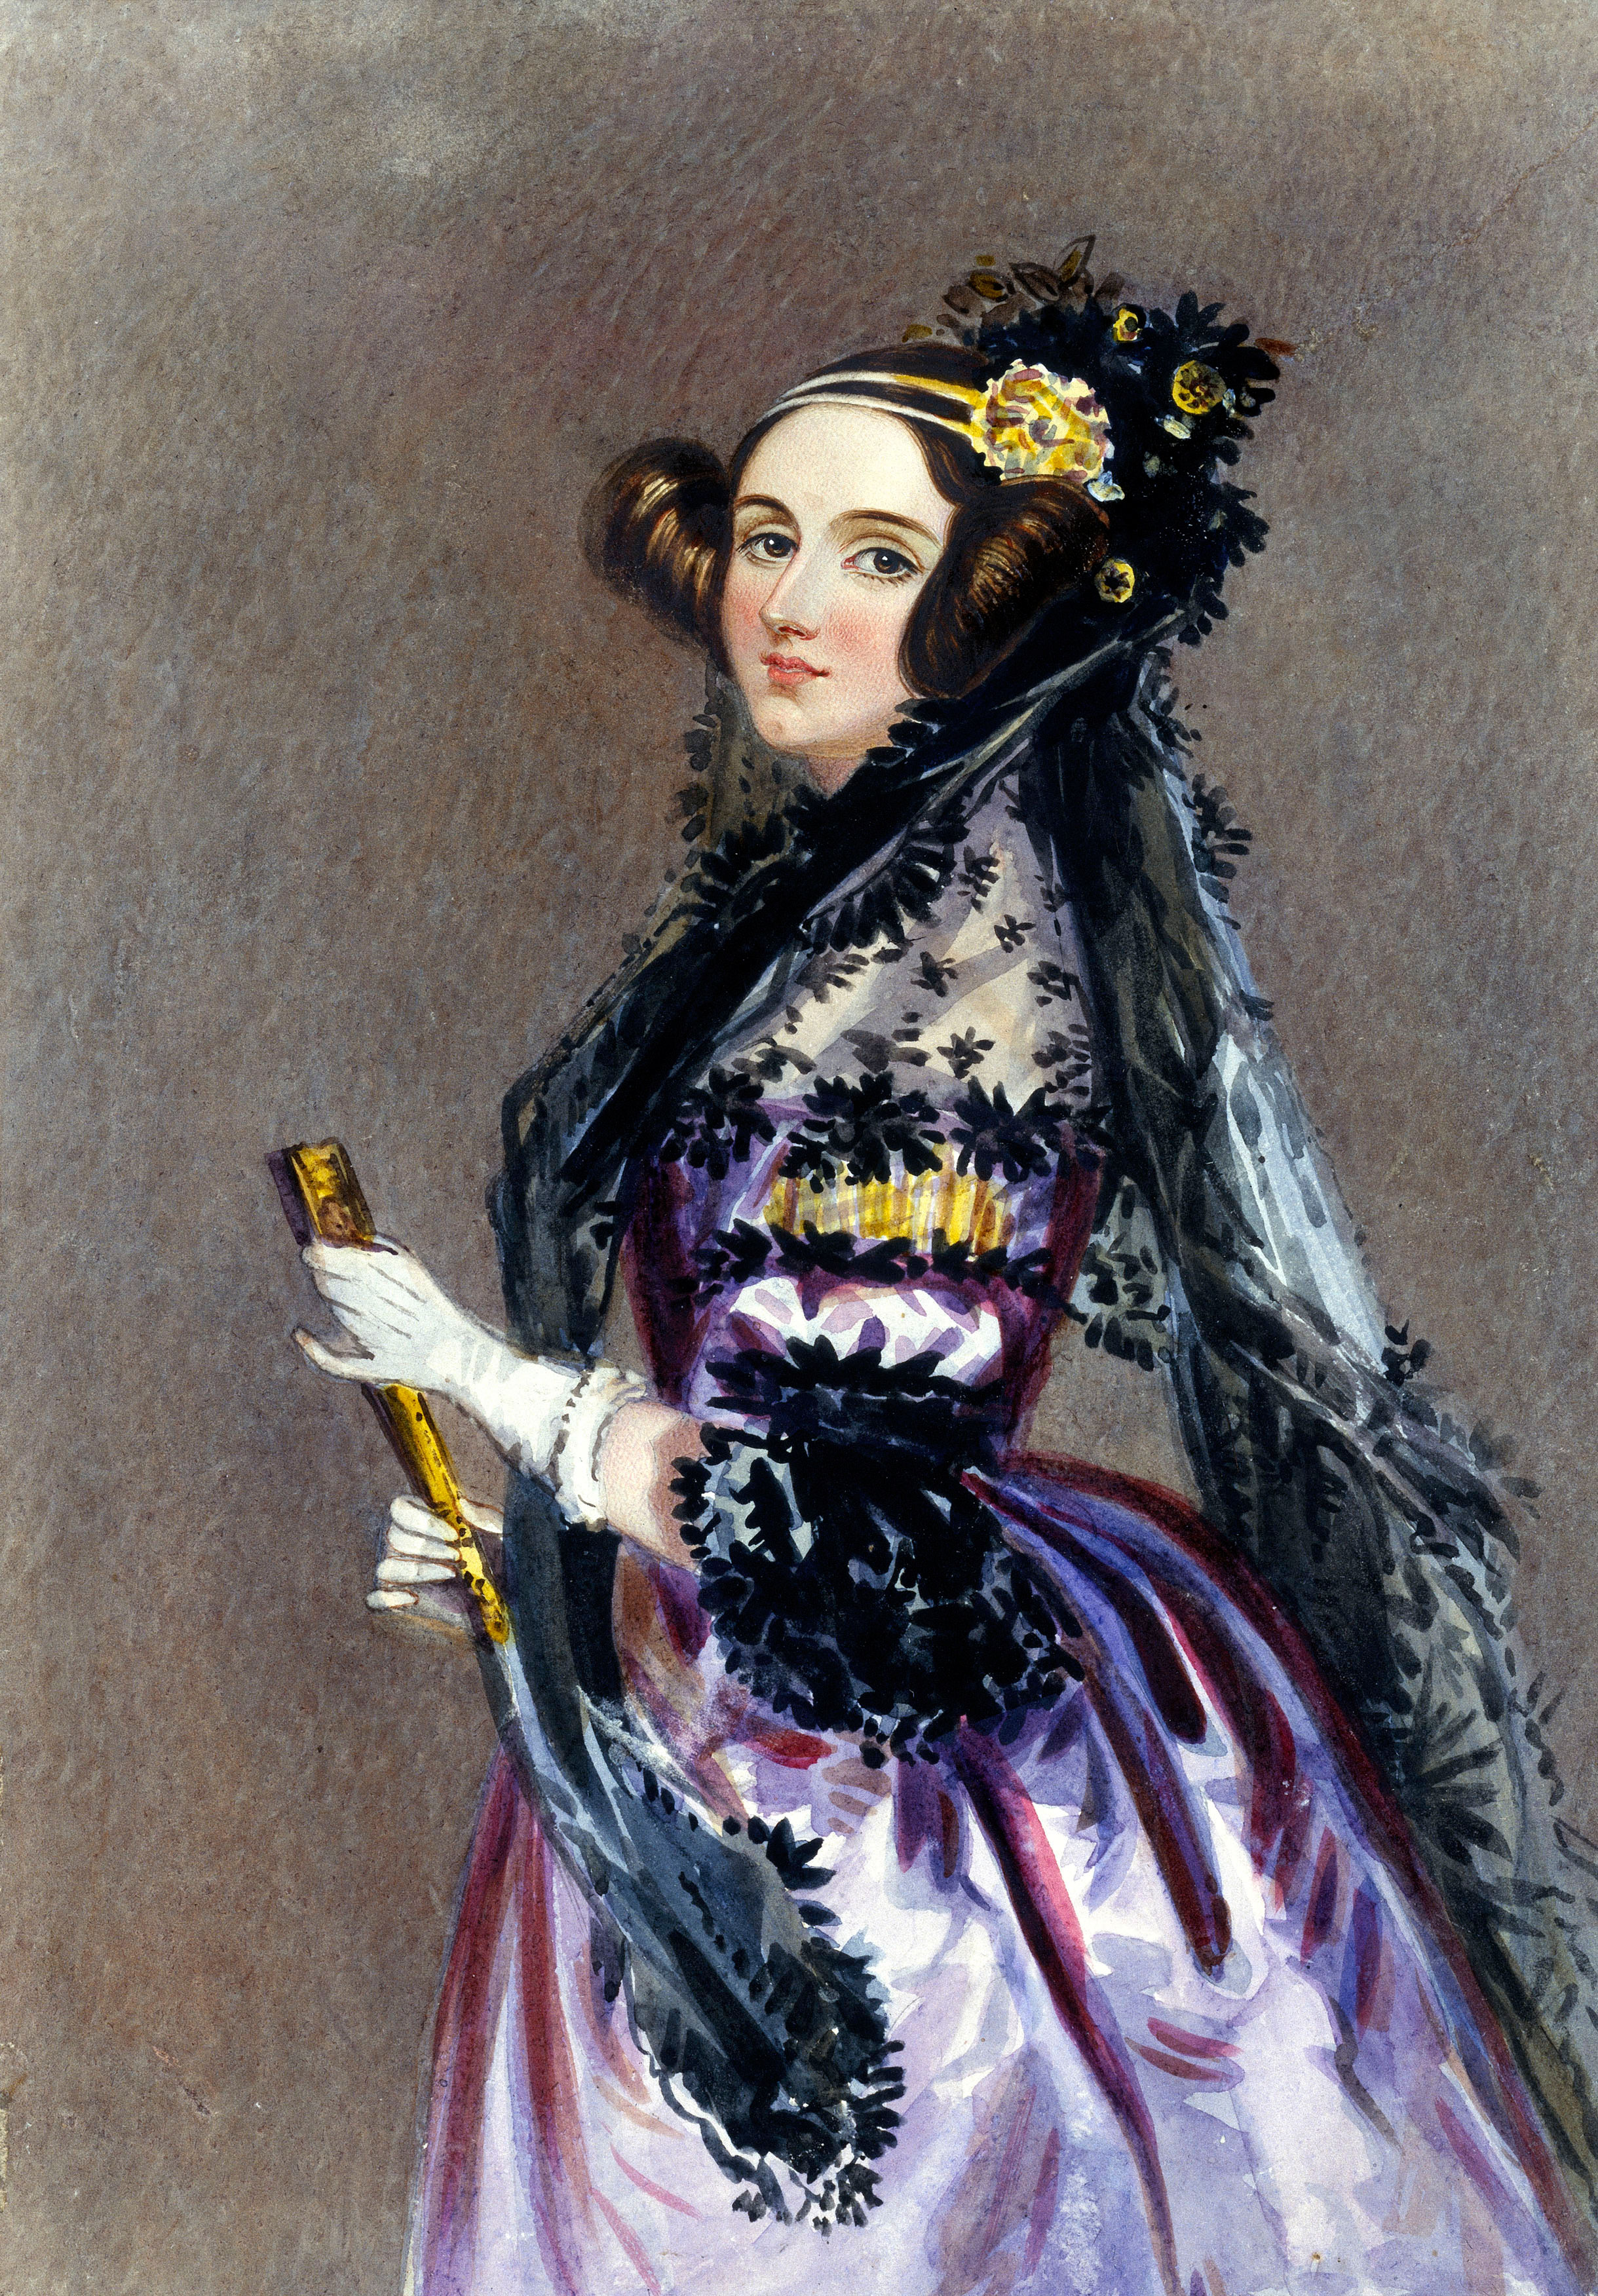
\includegraphics[width=0.4\linewidth]{graphics/Ada_Lovelace_portrait.jpg} % replace the path with your own file
\caption{The portrait of Ada Lovelace.}
\label{fig:ada}
\end{figure}    
\end{lstlisting}
\begin{figure}[ht!]
\centering
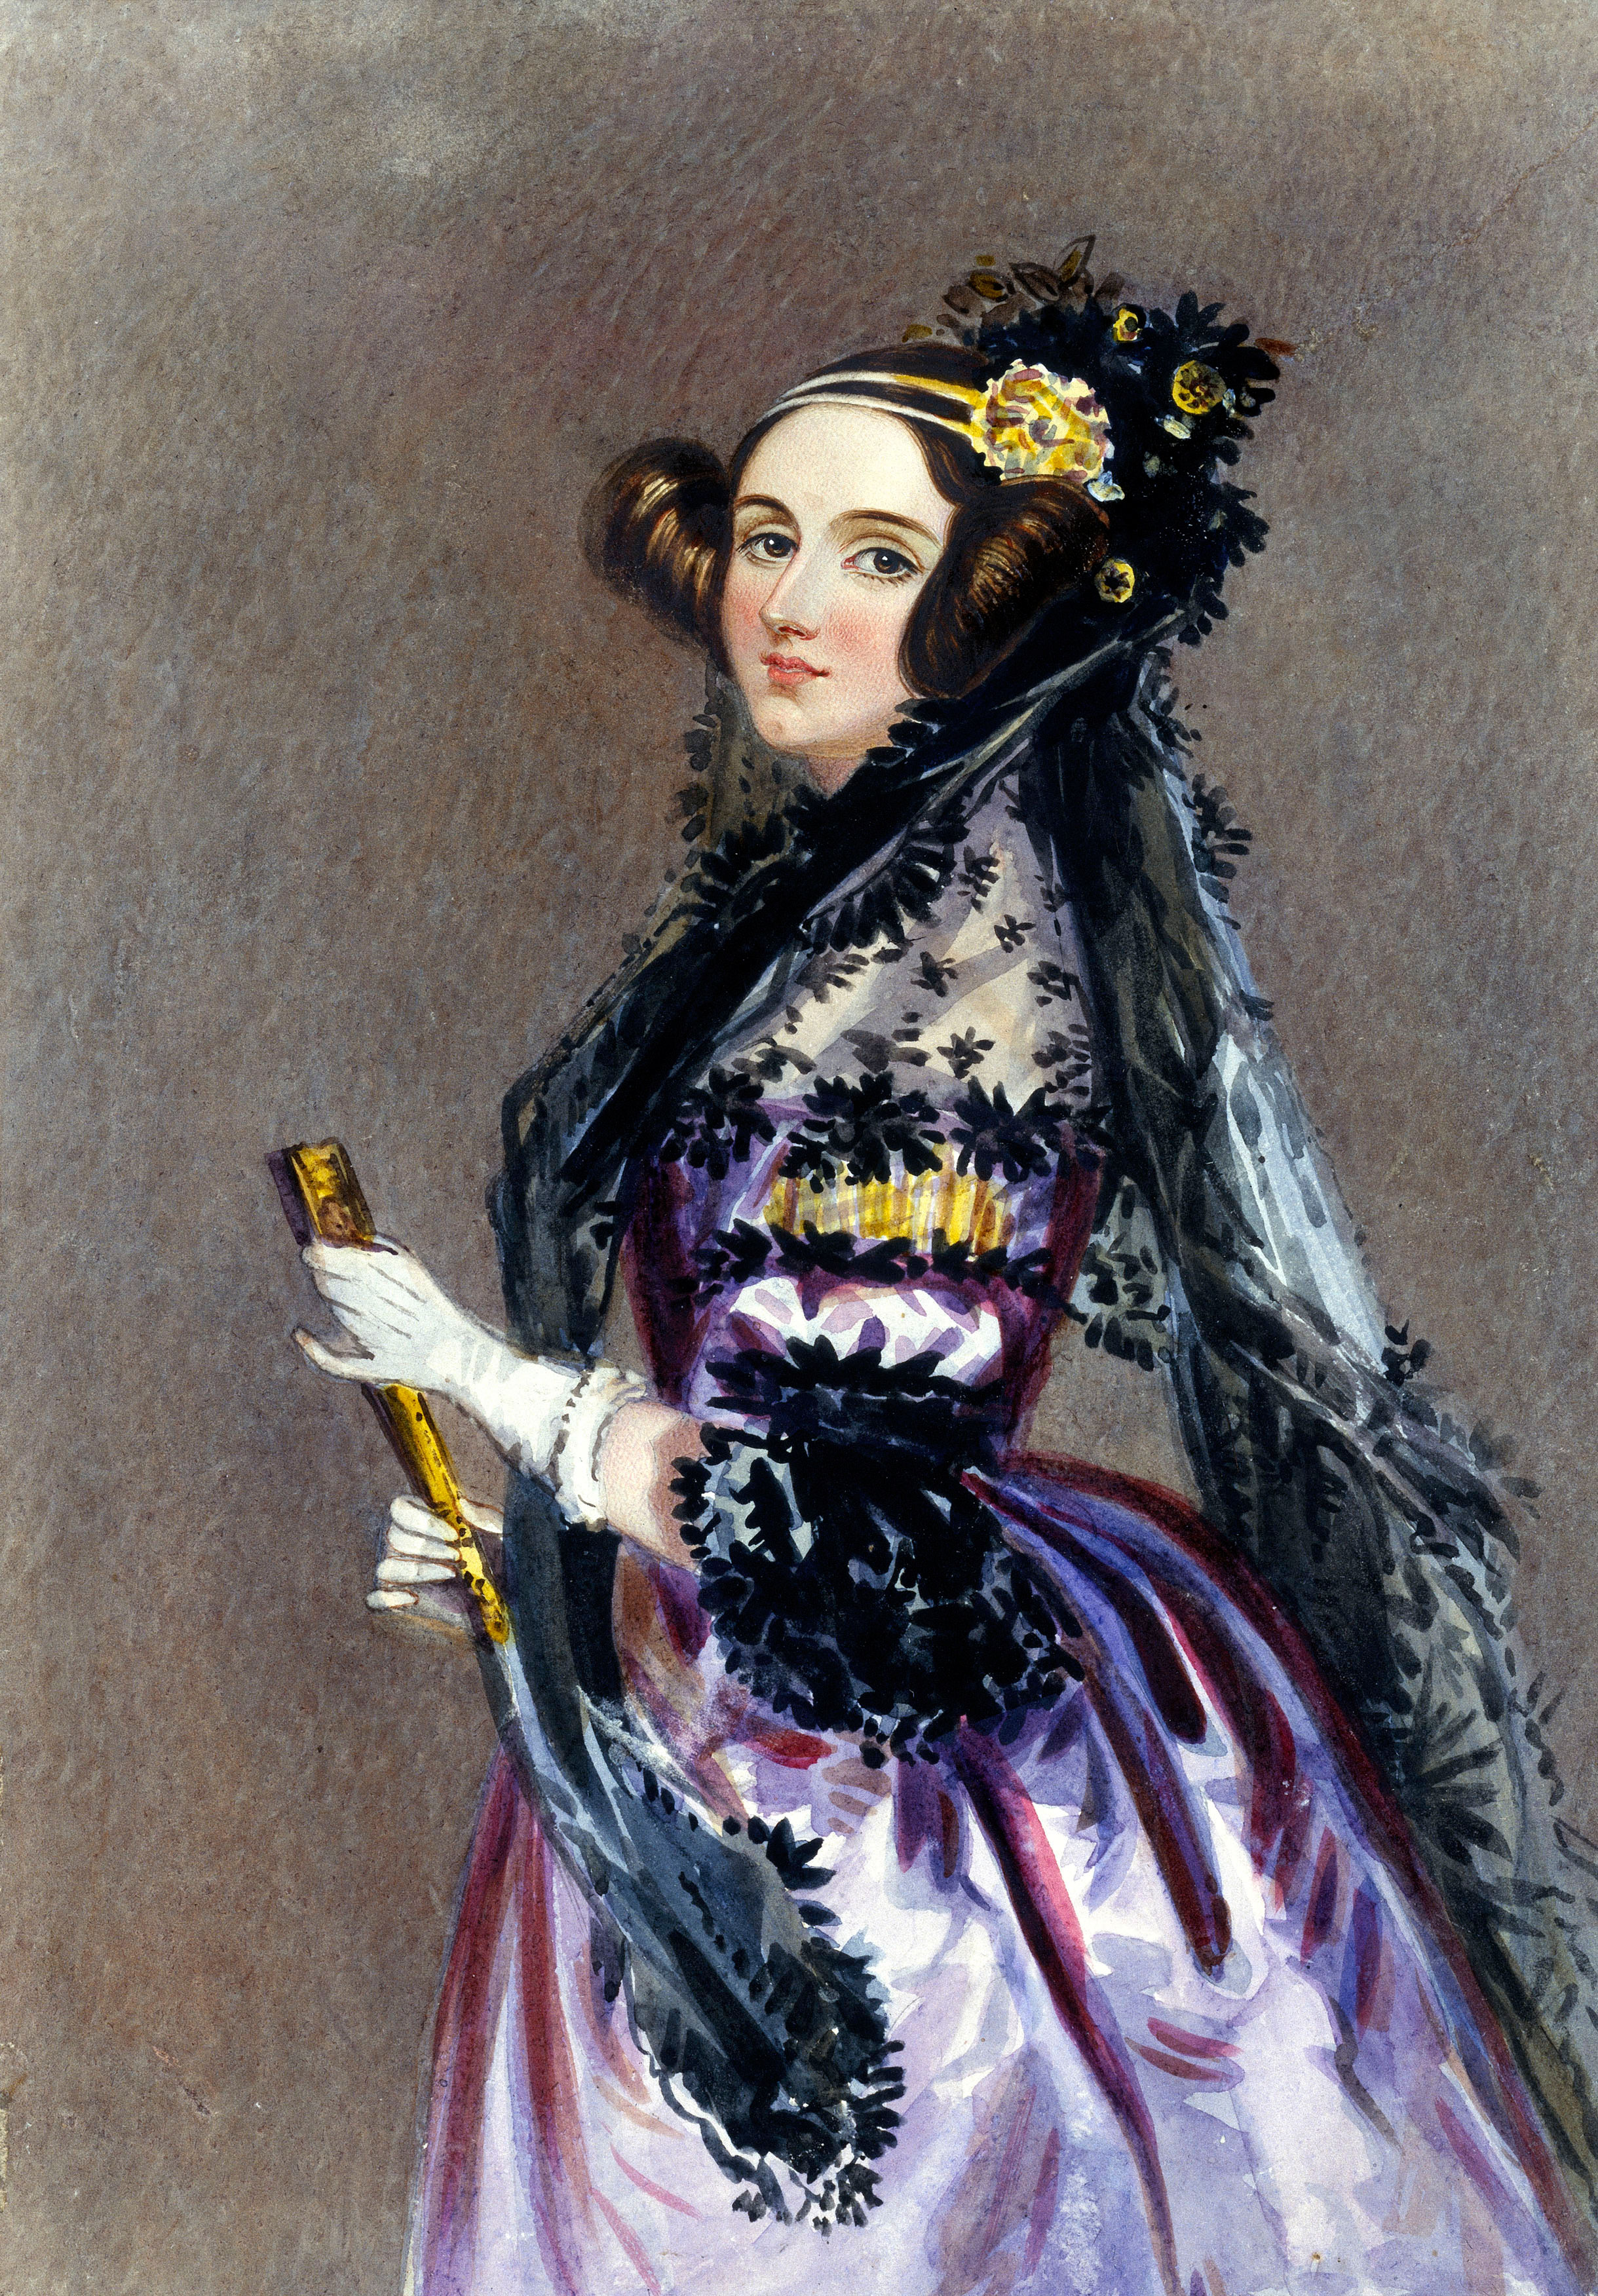
\includegraphics[width=0.4\linewidth]{graphics/Ada_Lovelace_portrait.jpg}
\caption{The portrait of Ada Lovelace.}
\label{fig:ada}
\end{figure}
First, we need to enclose the \texttt{\textbackslash includegraphics} command within a \verb|figure| environment. The \verb|ht!| option indicates that priority is given to put the figure structure exactly in the place where the code is inserted (\verb|h|: here), or at the top of a page (\verb|t|). The \verb|width| option enforces the width of the image to the input value (and similarly there are \verb|height| and \verb|scale|). The \verb|caption| command unsurprisingly generates the caption, while the \verb|label| command works as it is in math mode and allows us to reference it by writing \texttt{\textbackslash ref\{fig:ada\}}.

\paragraph{subcaption}
We can construct a set of subfigures within an overarching figure by utilizing the \verb|subcaption| package and \verb|subfigure| groups. To illustrate, the following code is deployed to generate Figure \ref{fig:TC1}: 
\begin{lstlisting}
\begin{figure}[ht!]
\centering
\begin{subfigure}[b]{0.45\textwidth}
\centering
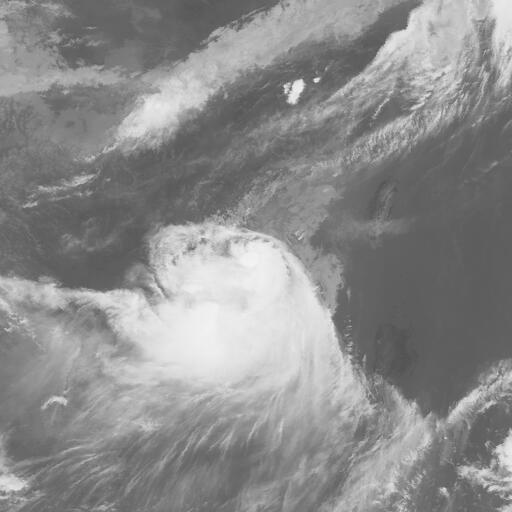
\includegraphics[width=0.8\linewidth]{graphics/MTS108082203.200812.jpg}
\caption{Typhoon Nuri (2008).}
\end{subfigure}
\begin{subfigure}[b]{0.45\textwidth}
\centering
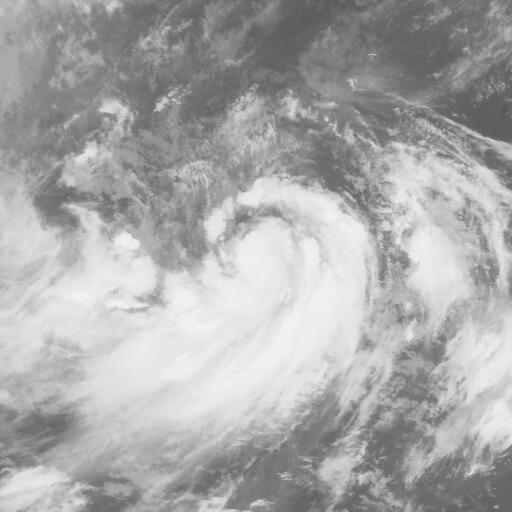
\includegraphics[width=0.8\linewidth]{graphics/MTS212072303.201208.jpg}
\caption{Typhoon Vicente (2012).}
\end{subfigure}
\caption{The infrared satellite images of various Tropical Cyclones affecting Hong Kong.}
\label{fig:TC1}
\end{figure}   
\end{lstlisting}
The \verb|b| option sets the vertical alignment of \verb|subfigure| at the bottom.

\begin{figure}[ht!]
\centering
\begin{subfigure}[b]{0.45\textwidth}
\centering
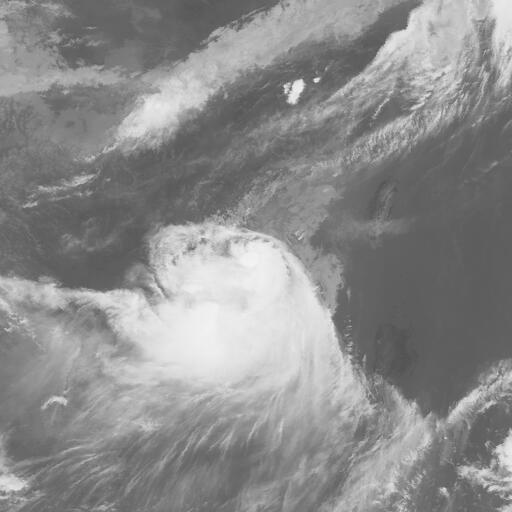
\includegraphics[width=0.8\linewidth]{graphics/MTS108082203.200812.jpg}
\caption{Typhoon Nuri (2008).}
\end{subfigure}
\begin{subfigure}[b]{0.45\textwidth}
\centering
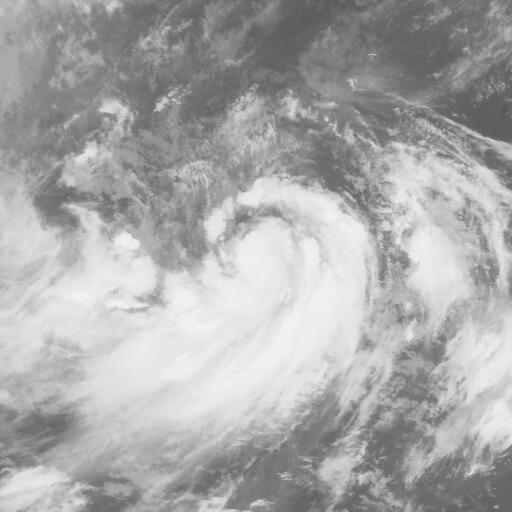
\includegraphics[width=0.8\linewidth]{graphics/MTS212072303.201208.jpg}
\caption{Typhoon Vicente (2012).}
\end{subfigure}
\caption{The infrared satellite images of various Tropical Cyclones affecting Hong Kong. (Source: \href{https://agora.ex.nii.ac.jp/digital-typhoon/index.html.en}{Digital Typhoon})}
\label{fig:TC1}
\end{figure}

\paragraph{ContinuedFloat} To make a longer figure of subfigures that spans multiple pages, we can simply arrange them into separate \verb|figure| environments and call the \texttt{\textbackslash ContinuedFloat} command in all the subsequent \verb|figure| groups. Continuing from the last example, we may have
\begin{lstlisting}
\begin{figure}[hb!]
\ContinuedFloat % here!
\caption{(Cont.) The infrared satellite images of various Tropical Cyclones affecting Hong Kong.}
\centering
\begin{subfigure}[b]{0.45\textwidth}
...
\caption{Typhoon Haima (2016).}
\end{subfigure}
...
\begin{subfigure}[b]{0.45\textwidth}
...
\caption{Typhoon Saola (2023).}
\end{subfigure}
\end{figure}    
\end{lstlisting}
producing
\begin{figure}[hb!]
\ContinuedFloat
\caption{(Cont.) The infrared satellite images of various Tropical Cyclones affecting Hong Kong.}
\centering
\begin{subfigure}[b]{0.45\textwidth}
\centering
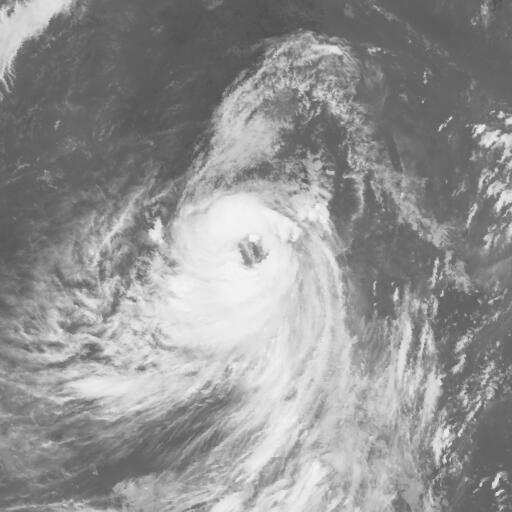
\includegraphics[width=0.8\linewidth]{graphics/HMW816080103.201604.jpg}
\caption{Typhoon Haima (2016).}
\end{subfigure}
\begin{subfigure}[b]{0.45\textwidth}
\centering
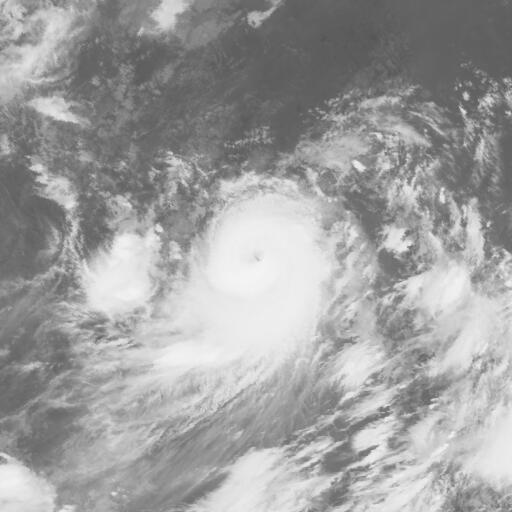
\includegraphics[width=0.8\linewidth]{graphics/HMW817082303.201713.jpg}
\caption{Typhoon Hato (2017).}
\end{subfigure}
\begin{subfigure}[b]{0.45\textwidth}
\centering
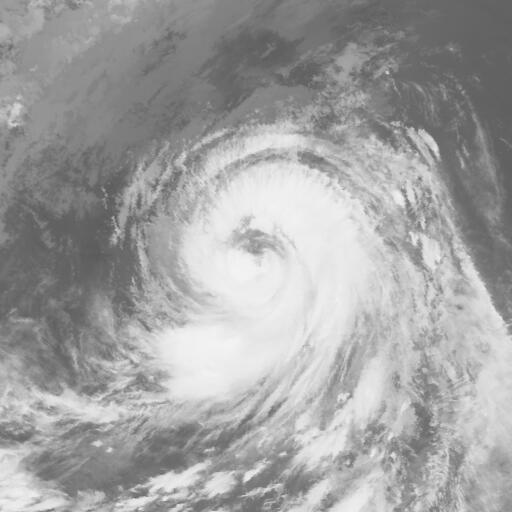
\includegraphics[width=0.8\linewidth]{graphics/HMW818091603.201822.jpg}
\caption{Typhoon Mangkhut (2018).}
\end{subfigure}
\begin{subfigure}[b]{0.45\textwidth}
\centering
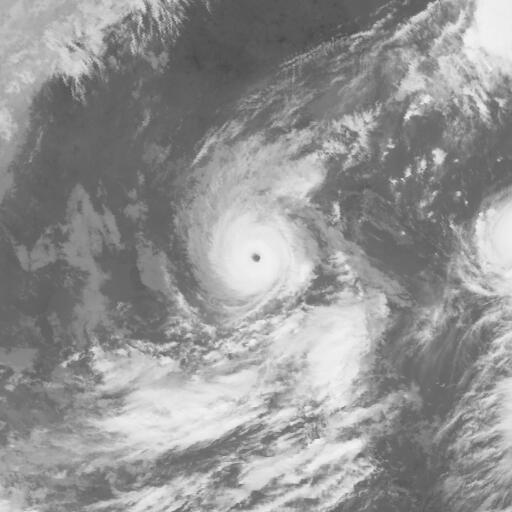
\includegraphics[width=0.8\linewidth]{graphics/HMW923090103.202309.jpg}
\caption{Typhoon Saola (2023).}
\end{subfigure}
\end{figure}

\subsection{Tables}

\paragraph{table, tabularx}
Just like embedding figures, building a table requires us to place the content inside the corresponding \verb|table| environment. While it is possible to use the native \verb|tabular| class for the actual table itself, a more powerful version is provided by the \verb|tabularx| package and its class that bears the same name. This is demonstrated via Table \ref{tab:armyunits} thereafter, which is generated by
\begin{lstlisting}
\begin{table}[ht!]
\centering
\begin{tabularx}{\textwidth}{|l|p{0.55\textwidth}|>{\raggedleft}X|>{\raggedleft\arraybackslash}X|}
\hline
Unit & Description & Attack & Defense \\
\hline
Infantry & The most basic unit and backbone of any army, all-around abilities with a cheap cost. & 20 & 25 \\
\hline
Cavalry & The shock unit in an army with very strong power. & 40 & 30 \\
\hline
Artillery & The support unit that provides bombardment support from far away. & 30 & 5 \\
\hline
\end{tabularx}
\caption{The unit statistics table for a hypothetical game.}
\label{tab:armyunits}
\end{table}
\end{lstlisting}
\begin{table}[ht!]
\centering
\begin{tabularx}{\textwidth}{|l|p{0.55\textwidth}|>{\raggedleft}X|>{\raggedleft\arraybackslash}X|}
\hline
Unit & Description & Attack & Defense \\
\hline
Infantry & The most basic unit and backbone of any army, all-around abilities with a cheap cost. & 20 & 25 \\
\hline
Cavalry & The shock unit in an army with very strong power. & 40 & 30 \\
\hline
Artillery & The support unit that provides bombardment support from far away. & 30 & 5 \\
\hline
\end{tabularx}
\caption{The unit statistics table for a hypothetical game.}
\label{tab:armyunits}
\end{table}
The \verb|ht!| option, \verb|caption|, and \verb|label| work exactly as the figure counterpart. For the \verb|tabularx| group, the first argument indicates the width of the entire table, set to \texttt{\textbackslash textwidth} here. The second argument \texttt{\{|l|p\{0.55\textbackslash textwidth\}|\allowbreak >\{\textbackslash raggedleft\}X|>\{\textbackslash raggedleft\textbackslash arraybackslash\}X|\}} indicates the justification of the columns: the first column is left-aligned (\verb|l|, similarly we have \verb|c| and \verb|r|) and its size will fit the text; the second column (\verb|p|) forces a width of $0.55$ times \texttt{\textbackslash textwidth}; the remaining width is distributed evenly to last two columns (\verb|X|). The part of \texttt{>\{\textbackslash raggedleft\}} is applied to the \verb|X| columns, making them right-aligned.\footnote{\texttt{\textbackslash arraybackslash} is needed in the last column, see \href{https://tex.stackexchange.com/questions/372464/last-tabularx-column-raggedright-with-memoir}{\TeX{} StackExchange 372464}.} Finally, \texttt{|} and \texttt{\textbackslash hline} produce vertical/horiztonal separating lines; \texttt{\&} slices between the columns and \texttt{\textbackslash\textbackslash} marks the end of a row.

Also, note that \texttt{\textbackslash ContinuedFloat} can also be applied to \texttt{table}.

\paragraph{captionbeside} It is also possible to arrange the table so that the caption appears to the side of it. This is done by stacking the \verb|captionbeside| environment provided by KOMA-script. For example, the code
\begin{lstlisting}
\begin{table}[ht]
\begin{captionbeside}{This caption appears to the left of the Fibonacci numbers table.}[l][\textwidth]{
\adjustbox{valign=t}{
    \begin{tabularx}{0.4\textwidth}{|X|X|}
    \hline
    $n$ & $F_n$ \\
    \hline 
    $1$ & $1$ \\
    \hline 
    $2$ & $1$ \\
    \hline 
    $3$ & $2$ \\
    \hline 
    $4$ & $3$ \\
    \hline
    $5$ & $5$ \\
    \hline
    $6$ & $8$ \\
    \hline
    \end{tabularx}}
}
\end{captionbeside}
\label{tab:fib}
\end{table}    
\end{lstlisting}
produces Table \ref{tab:fib} below.

\begin{table}[ht]
\begin{captionbeside}{This caption appears to the left of the Fibonacci numbers table.}[l][\textwidth]{\adjustbox{valign=t}{\begin{tabularx}{0.4\textwidth}{|X|X|}
\hline
$n$ & $F_n$ \\
\hline 
$1$ & $1$ \\
\hline 
$2$ & $1$ \\
\hline 
$3$ & $2$ \\
\hline 
$4$ & $3$ \\
\hline
$5$ & $5$ \\
\hline
$6$ & $8$ \\
\hline
\end{tabularx}}}
\end{captionbeside}
\label{tab:fib}
\end{table}
We fill the caption in the first argument, followed by the relative position of the caption (\verb|l|: left) and the full width of the structure, finally with the actual \verb|tabularx| object. We also have to additionally load the \verb|adjustbox| package and use the corresponding command to tell the table to align itself at the top (\verb|valign=t|). This also requires us to first set the \texttt{\textbackslash KOMAoptions} to take \verb|captions=besidetop| (likewise we have \verb|captions=besidebottom| and more).

\paragraph{Shared Numbering between Figures and Tables}
Sometimes we may want to share the numbering between \textit{floats} (including figures, tables, and so on). This is done by the following patch that can be inserted into the preamble:
\begin{lstlisting}
\makeatletter
\let\c@table\c@figure
\let\ftype@table\ftype@figure
\makeatother
\end{lstlisting}
This involves the primitive \TeX{} functions, so we will not discuss them there. For more information, read \href{https://stackoverflow.com/questions/3865036/using-a-single-count-for-figures-and-tables-in-latex}{StackOverflow 3865036}, and \href{https://tex.stackexchange.com/questions/8351/what-do-makeatletter-and-makeatother-do}{\TeX{} StackExchange 8351} for what the \texttt{\textbackslash makeatletter} and \texttt{\textbackslash makeatother} commands do.

\begin{exercisebox}
\begin{Exercise}
Try to import and load your favorite image into the document. 
\end{Exercise}
\begin{Exercise}
Recreate any one of the tables in Chapter \ref{chap:maths}.
\end{Exercise}
\end{exercisebox}

\section{Minipages and Multiple Columns}

\paragraph{minipage}
Sometimes we may want to partition the content into smaller blocks that are embedded within the current page, and can be placed or ordered (e.g.\ parallel) in the way we want. The \verb|minipage| environment basically acts like a more versatile version of a \verb|parbox| environment and serves this purpose. For example, something like
\begin{lstlisting}
yields \par
\begin{center}
\begin{minipage}[b]{0.48\textwidth}
\lipsum[6]
\end{minipage}
\hfill
\begin{minipage}[b]{0.48\textwidth}
\lipsum[7]
\end{minipage}    
\end{center}      
\end{lstlisting}
yields \par
\begin{center}
\begin{minipage}[b]{0.48\textwidth}
\lipsum[6]
\end{minipage}
\hfill
\begin{minipage}[b]{0.48\textwidth}
\lipsum[7]
\end{minipage}    
\end{center}
The \verb|[b]| option indicates the baseline is set at the bottom, and hence the two blocks will be bottom-aligned, provided that their width is fixed to $0.48$ times \texttt{\textbackslash textwidth} and thus they fit in the main text area.

\paragraph{parcolumns} The \verb|parcolumns| package can also achieve the above effect and is more specialized for typesetting different pieces in two or more parallel columns. It also supports page breaks. Using the same example, we can write
\begin{lstlisting}
\begin{parcolumns}{2}
\colchunk[1]{\lipsum[6]}
\colchunk[2]{\lipsum[7]}
\colplacechunks
\colchunk[1]{\lipsum[8]}
\colchunk[2]{\lipsum[9]}
\end{parcolumns}
\end{lstlisting}
to get\\
\begin{parcolumns}{2}
\colchunk[1]{\lipsum[6]}
\colchunk[2]{\lipsum[7]}
\colplacechunks
\colchunk[1]{\lipsum[8]}
\colchunk[2]{\lipsum[9]}
\end{parcolumns}
where the first argument of the environment clearly indicates the number of columns and the \texttt{\textbackslash colplacechunks} command releases the loaded \texttt{\textbackslash colchunk[<col\allowbreak\_no.>]} and goes to the next paragraph.

\paragraph{multicol} A task closely related to what \verb|parcolumns| does above is to typeset a single, continuous stream of text along multiple columns, like in many academic papers. The \texttt{multicol} package is designed for this and will carry out the automatic splitting. For example, by encapsulating the text inside the \verb|multicols| environment as
\begin{lstlisting}
\begin{multicols}{2}
Zhuge Liang (born 181, Yangdu [now Yinan, Shandong province], China--died August 234, Wuzhangyuan [now in Shaanxi province], China) was a celebrated adviser to Liu Bei, founder of the Shu-Han dynasty (221--263/264).
...
A mechanical and mathematical genius, Zhuge is credited with inventing a bow for shooting several arrows at once and with perfecting the Eight Dispositions, a series of military tactics. In the Sanguozhi yanyi (Romance of the Three Kingdoms), the great 14th-century historical novel, Zhuge is one of the main characters; he is portrayed as being able to control the wind and foretell the future.
\end{multicols}
\end{lstlisting}
(again with the number of columns indicated in the first argument) we may acquire the following layout:
\begin{multicols}{2}
Zhuge Liang (born 181, Yangdu [now Yinan, Shandong province], China--died August 234, Wuzhangyuan [now in Shaanxi province], China) was a celebrated adviser to Liu Bei, founder of the Shu-Han dynasty (221--263/264).

Quick Facts: \\
Wade-Giles romanization: Chu-ko Liang \\
Courtesy name: Kongming \\
Born: 181, Yangdu [now Yinan, Shandong province], China \\
Died: August 234, Wuzhangyuan [now in Shaanxi province], China (aged 53)

Zhuge, to whom supernatural powers often are ascribed, has been a favoured character of many Chinese plays and stories. Legend states that Liu Bei, then a minor military figure, heard of Zhuge Liang’s great wisdom and came three times to the wilderness retreat to which Zhuge had retired to seek him out as an adviser. It is known that Zhuge helped Liu organize a large army and found a dynasty. Liu was so impressed with Zhuge’s wisdom that on his deathbed Liu urged his son to depend on Zhuge’s advice and urged Zhuge to ascend the throne himself if the prince were unable to rule. Some historical accounts indicate that Zhuge died from illness while leading a military campaign in 234.

A mechanical and mathematical genius, Zhuge is credited with inventing a bow for shooting several arrows at once and with perfecting the Eight Dispositions, a series of military tactics. In the Sanguozhi yanyi (Romance of the Three Kingdoms), the great 14th-century historical novel, Zhuge is one of the main characters; he is portrayed as being able to control the wind and foretell the future. (Source: Encyclopaedia Britannica)
\end{multicols}


\paragraph{twocolumn} We can also pass the \verb|twocolumn=true| option to \texttt{\textbackslash KOMAoptions} to demand the entire book to be formatted in two columns globally. However, note that it will greatly mess up the layout of this book. (The decision to adopt such a format should be made at an early time!)
\chapter{Self-defined Commands and Environments}

\section{Self-defined Commands}

\section{If-then-else Statements}

\section{Self-defined Environments}

\chapter{More on Book Layout Design}
\chapter{Framed Theorems and Exercises}
\chapter{Plotting with Tikz}
\chapter{Miscellaneous}

\end{document}
